% Nội dung phần 3: Kết quả phân tích và mô hình hóa.
% Theo yêu cầu đề bài, phần này chỉ trình bày bảng kết quả, biểu đồ và diễn giải;
% toàn bộ mã R nằm trong file de_xuat_phan_tich_clickstream.Rmd.

\section{Kết quả phân tích và mô hình hóa}
\label{sec:results}

\subsection{Kết quả so sánh hai nhóm giá dạng A/B}
\label{subsec:ab}

Phân tích chính được thực hiện trên tập validation tháng 7 (35.231 click của
5.071 session). Nhóm A gồm các click vào sản phẩm \emph{không} có giá cao hơn
trung bình danh mục; nhóm B gồm các click vào sản phẩm có giá cao hơn trung bình
danh mục.

\subsubsection{Kết quả kiểm định}

\begin{table}[H]
\centering
\caption{Tỷ lệ Exit theo nhóm giá trên tập validation tháng 7}
\label{tab:ab-rate}
\small
\begin{tabular}{lrrrrl}
\toprule
\textbf{Nhóm} & \textbf{Click} & \textbf{Session} & \textbf{Exit}
& \textbf{Tỷ lệ Exit} & \textbf{CI 95\% (Wilson)} \\
\midrule
A: Không cao hơn TB & 16.879 & 4.147 & 2.325 & 13,77\% & 13,26\% -- 14,30\% \\
B: Cao hơn TB       & 18.352 & 4.249 & 2.746 & 14,96\% & 14,45\% -- 15,49\% \\
\bottomrule
\end{tabular}
\end{table}

Một session có thể xem sản phẩm thuộc cả hai nhóm giá, nên tổng số session ở hai
hàng của Bảng~\ref{tab:ab-rate} lớn hơn 5.071 và không được cộng lại.

\begin{table}[H]
\centering
\caption{Tổng hợp các kiểm định so sánh hai nhóm giá (tháng 7)}
\label{tab:ab-test}
\small
\begin{tabular}{>{\raggedright\arraybackslash}p{0.30\textwidth}rll}
\toprule
\textbf{Đại lượng} & \textbf{Ước lượng} & \textbf{CI 95\%} & \textbf{p-value} \\
\midrule
Chênh lệch thô B $-$ A (điểm \%)      & 1,19  & 0,46 -- 1,93 (cluster bootstrap) & --- \\
Kiểm định hai tỷ lệ ($\chi^2$, df = 1) & 10,08 & ---                              & 0,002 \\
Adjusted odds ratio (B so với A)       & 1,071 & 1,002 -- 1,144 (robust)          & 0,043 \\
Adjusted risk difference (điểm \%)     & 0,82  & 0,03 -- 1,62 (robust)            & --- \\
Tương tác nhóm giá $\times$ Category   & ---   & ---                              & 0,051 \\
\bottomrule
\end{tabular}
\end{table}

Ở mức ý nghĩa 5\%, cả kiểm định hai tỷ lệ thô ($p = 0{,}002$) lẫn adjusted odds
ratio với sai số chuẩn cluster-robust theo session ($p = 0{,}043$) đều cho phép
\textbf{bác bỏ $H_0$}. Tuy nhiên độ lớn hiệu ứng rất khiêm tốn: sau khi điều
chỉnh tiến trình session, thời gian, country và toàn bộ đặc điểm sản phẩm, chênh
lệch xác suất chuẩn hóa chỉ còn 0,82 điểm phần trăm, với cận dưới của khoảng tin
cậy sát 0 (0,03 điểm phần trăm). Nói cách khác, bằng chứng về sự \emph{tồn tại}
của khác biệt là có, nhưng khác biệt đó nhỏ và ước lượng kém chính xác.

\begin{figure}[H]
\centering
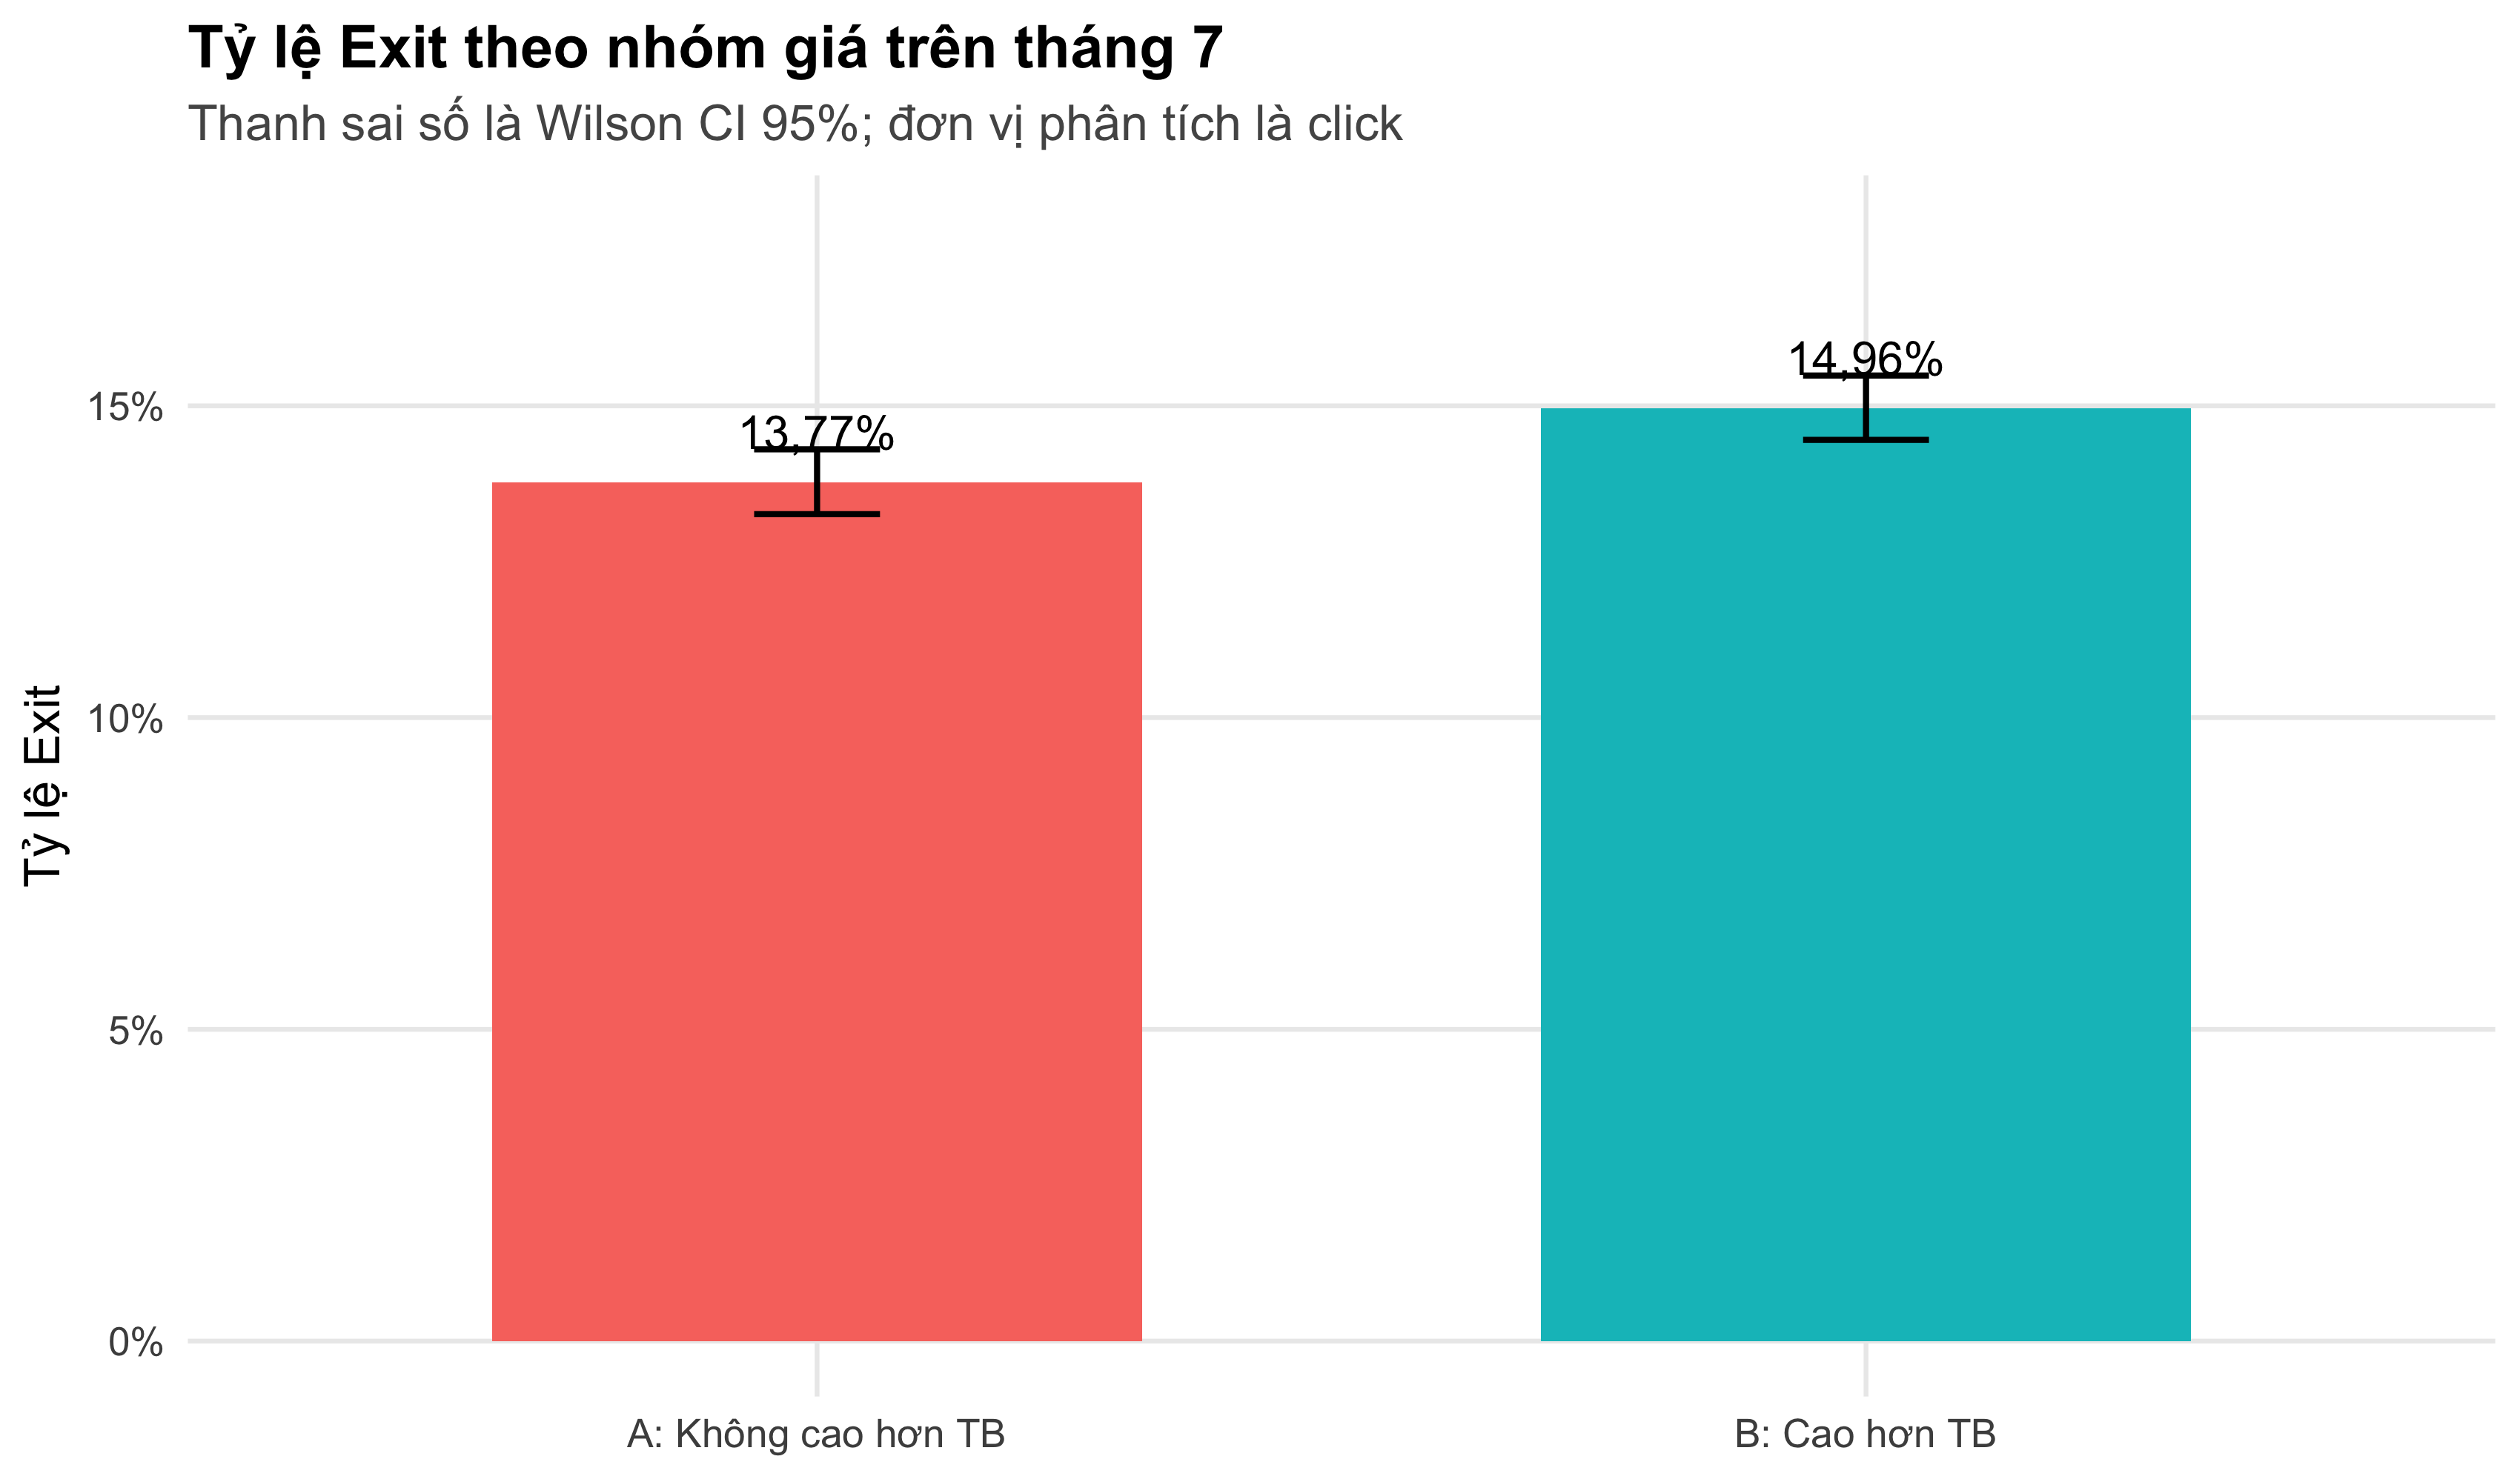
\includegraphics[width=0.8\textwidth]{img/fig-ab-exit-rate.png}
\caption{So sánh tỷ lệ Exit giữa hai nhóm giá trên tháng 7, thanh sai số là
khoảng tin cậy Wilson 95\%}
\label{fig:ab-exit-rate}
\end{figure}

\subsubsection{Kiểm tra balance giữa hai nhóm}

\begin{figure}[H]
\centering
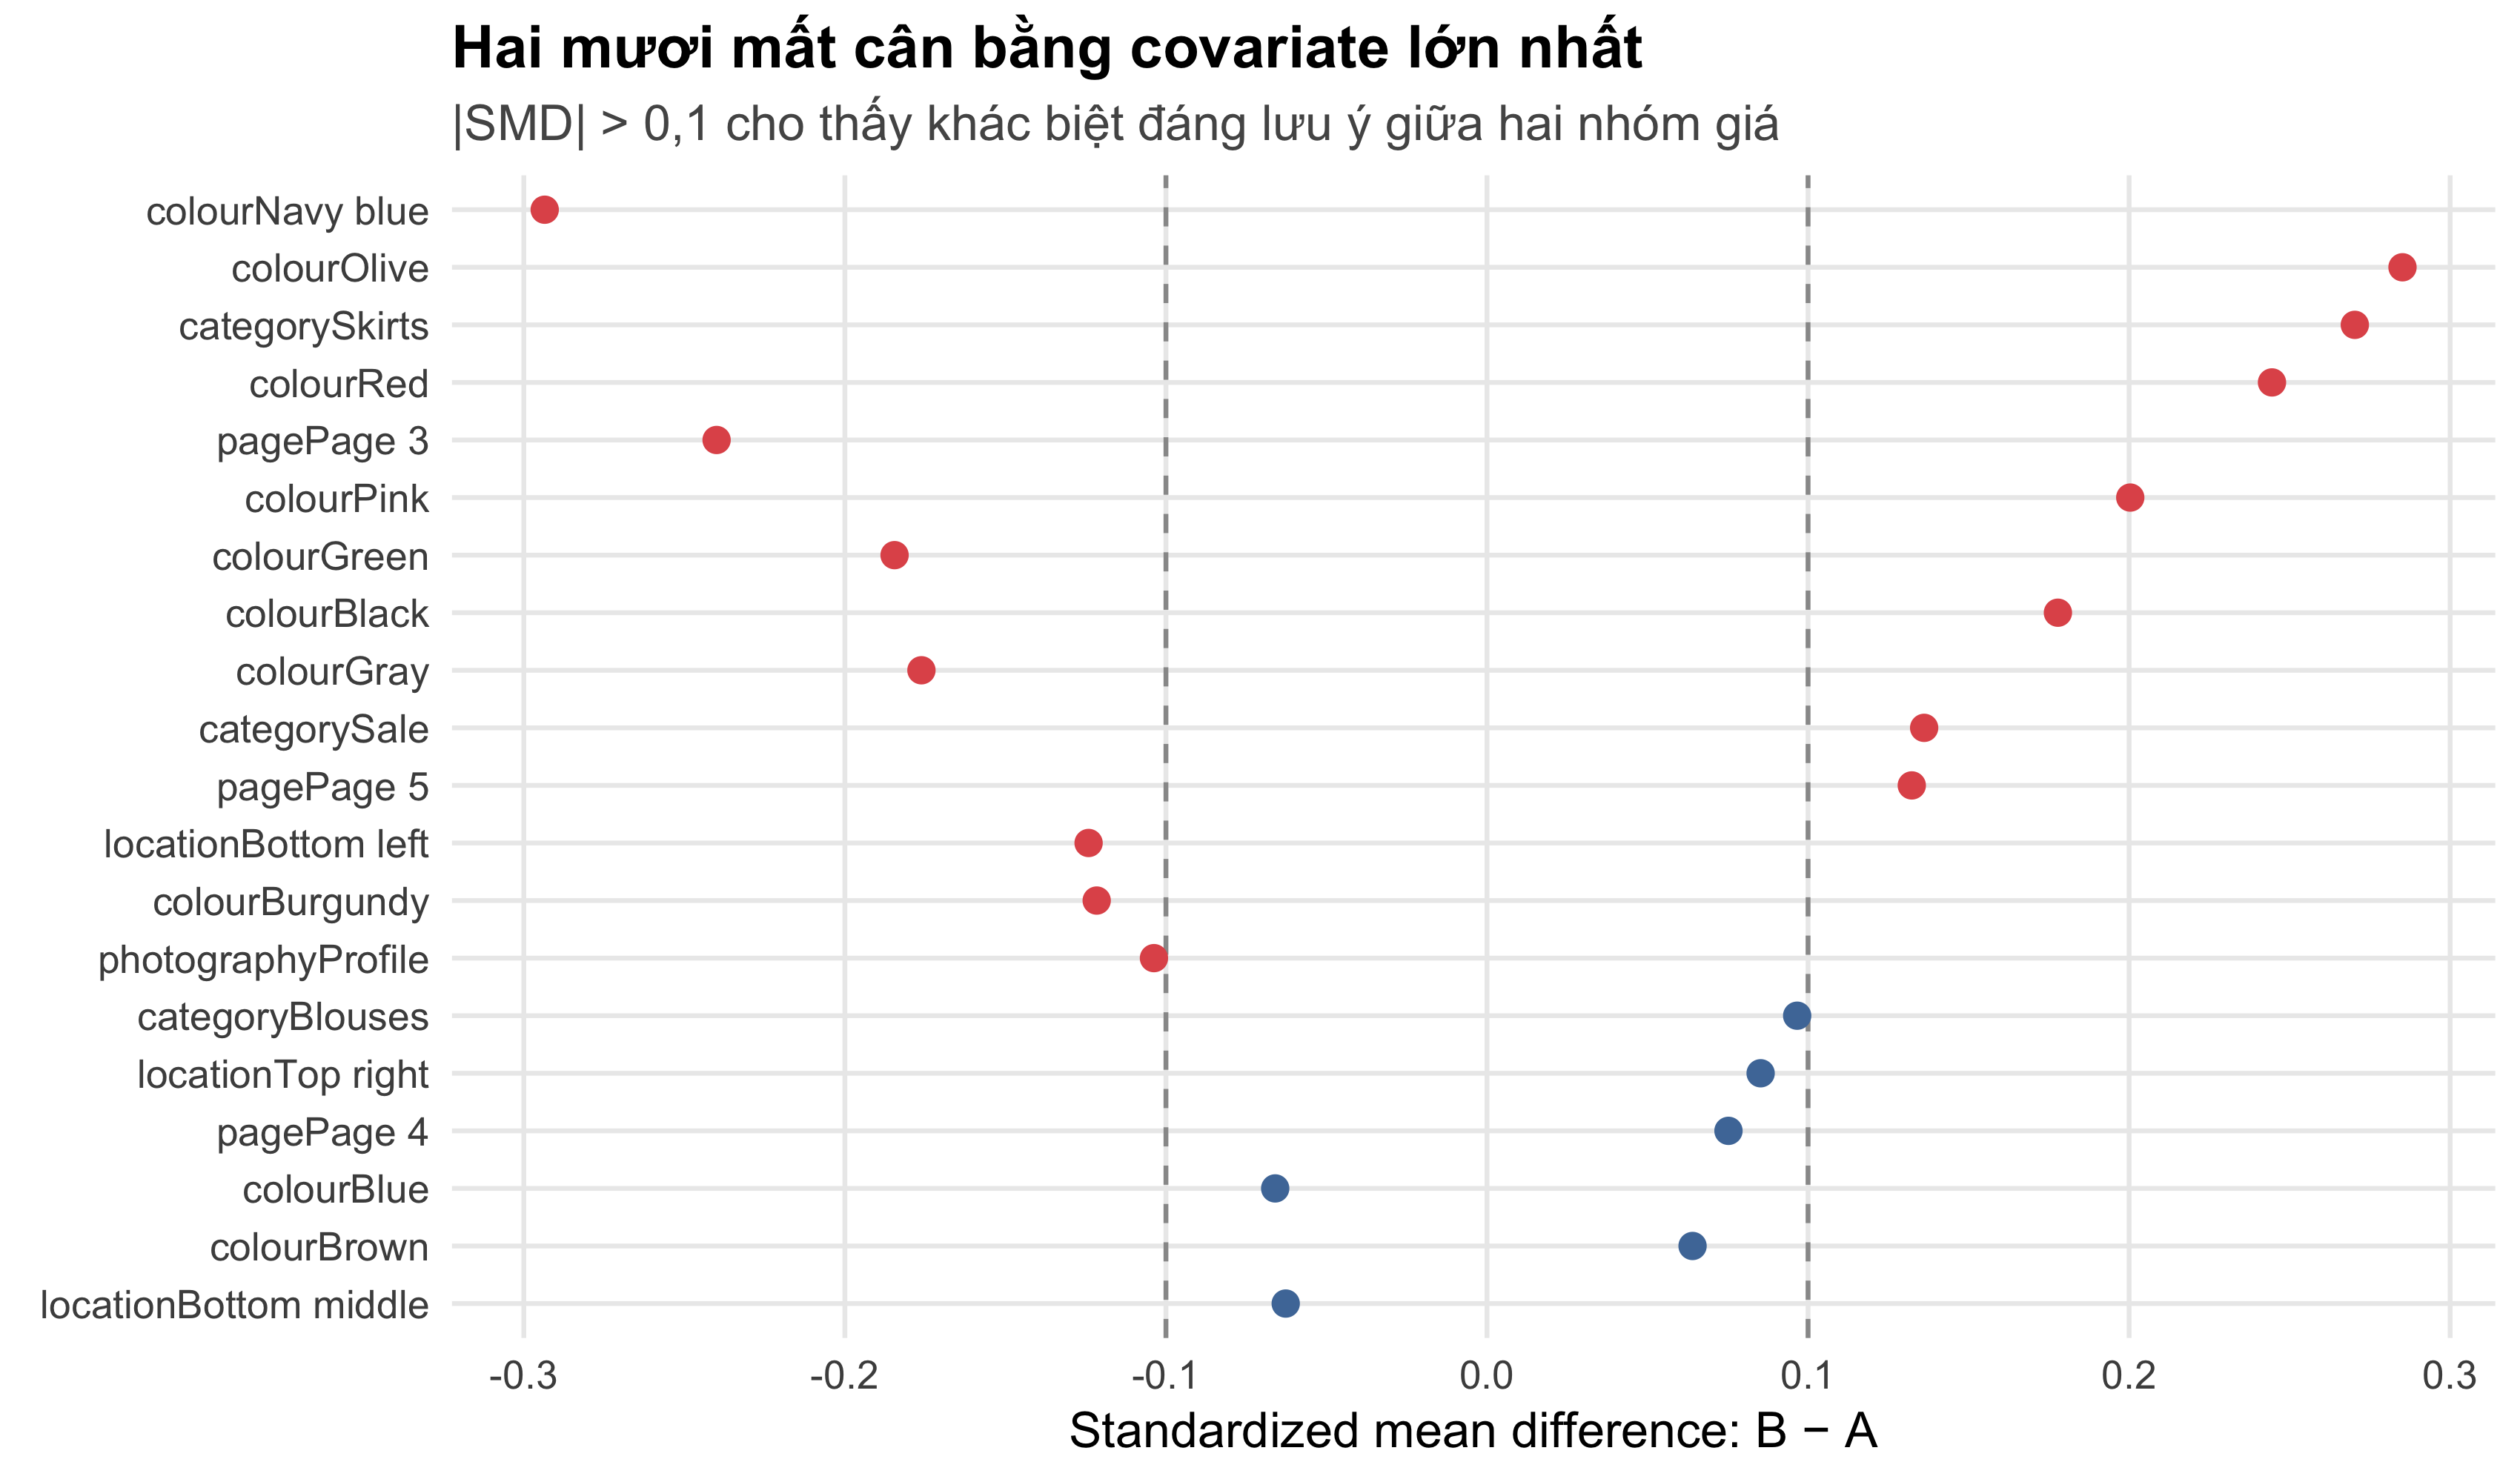
\includegraphics[width=\textwidth]{img/fig-ab-balance.png}
\caption{Hai mươi covariate mất cân bằng nhất giữa hai nhóm giá}
\label{fig:ab-balance}
\end{figure}

Hình~\ref{fig:ab-balance} là bằng chứng trực tiếp cho thấy hai nhóm \emph{không}
tương đương như trong một thí nghiệm ngẫu nhiên: nhiều covariate có
$|\text{SMD}| > 0{,}1$. Đây là lý do báo cáo ưu tiên adjusted risk difference và
suy luận robust thay vì chênh lệch thô. Dù vậy, việc điều chỉnh chỉ xử lý được
các yếu tố \emph{đã quan sát}; residual confounding vẫn có thể tồn tại.

\subsubsection{Dị biệt hiệu ứng theo danh mục}

\begin{table}[H]
\centering
\caption{Adjusted risk difference của nhóm giá theo từng danh mục (tháng 7)}
\label{tab:ab-category}
\small
\begin{tabular}{lrrll}
\toprule
\textbf{Category} & \textbf{N} & \textbf{Adjusted RD (điểm \%)}
& \textbf{CI 95\%} & \textbf{p-value (Holm)} \\
\midrule
Trousers & 10.871 & 2,32          & 0,86 -- 3,78            & 0,008 \\
Skirts   & 7.382  & 0,69          & $-$1,25 -- 2,62         & 1,000 \\
Blouses  & 7.858  & 0,72          & $-$0,88 -- 2,33         & 1,000 \\
Sale     & 9.120  & $-$0,66       & $-$2,17 -- 0,85         & 1,000 \\
\bottomrule
\end{tabular}
\end{table}

\begin{figure}[H]
\centering
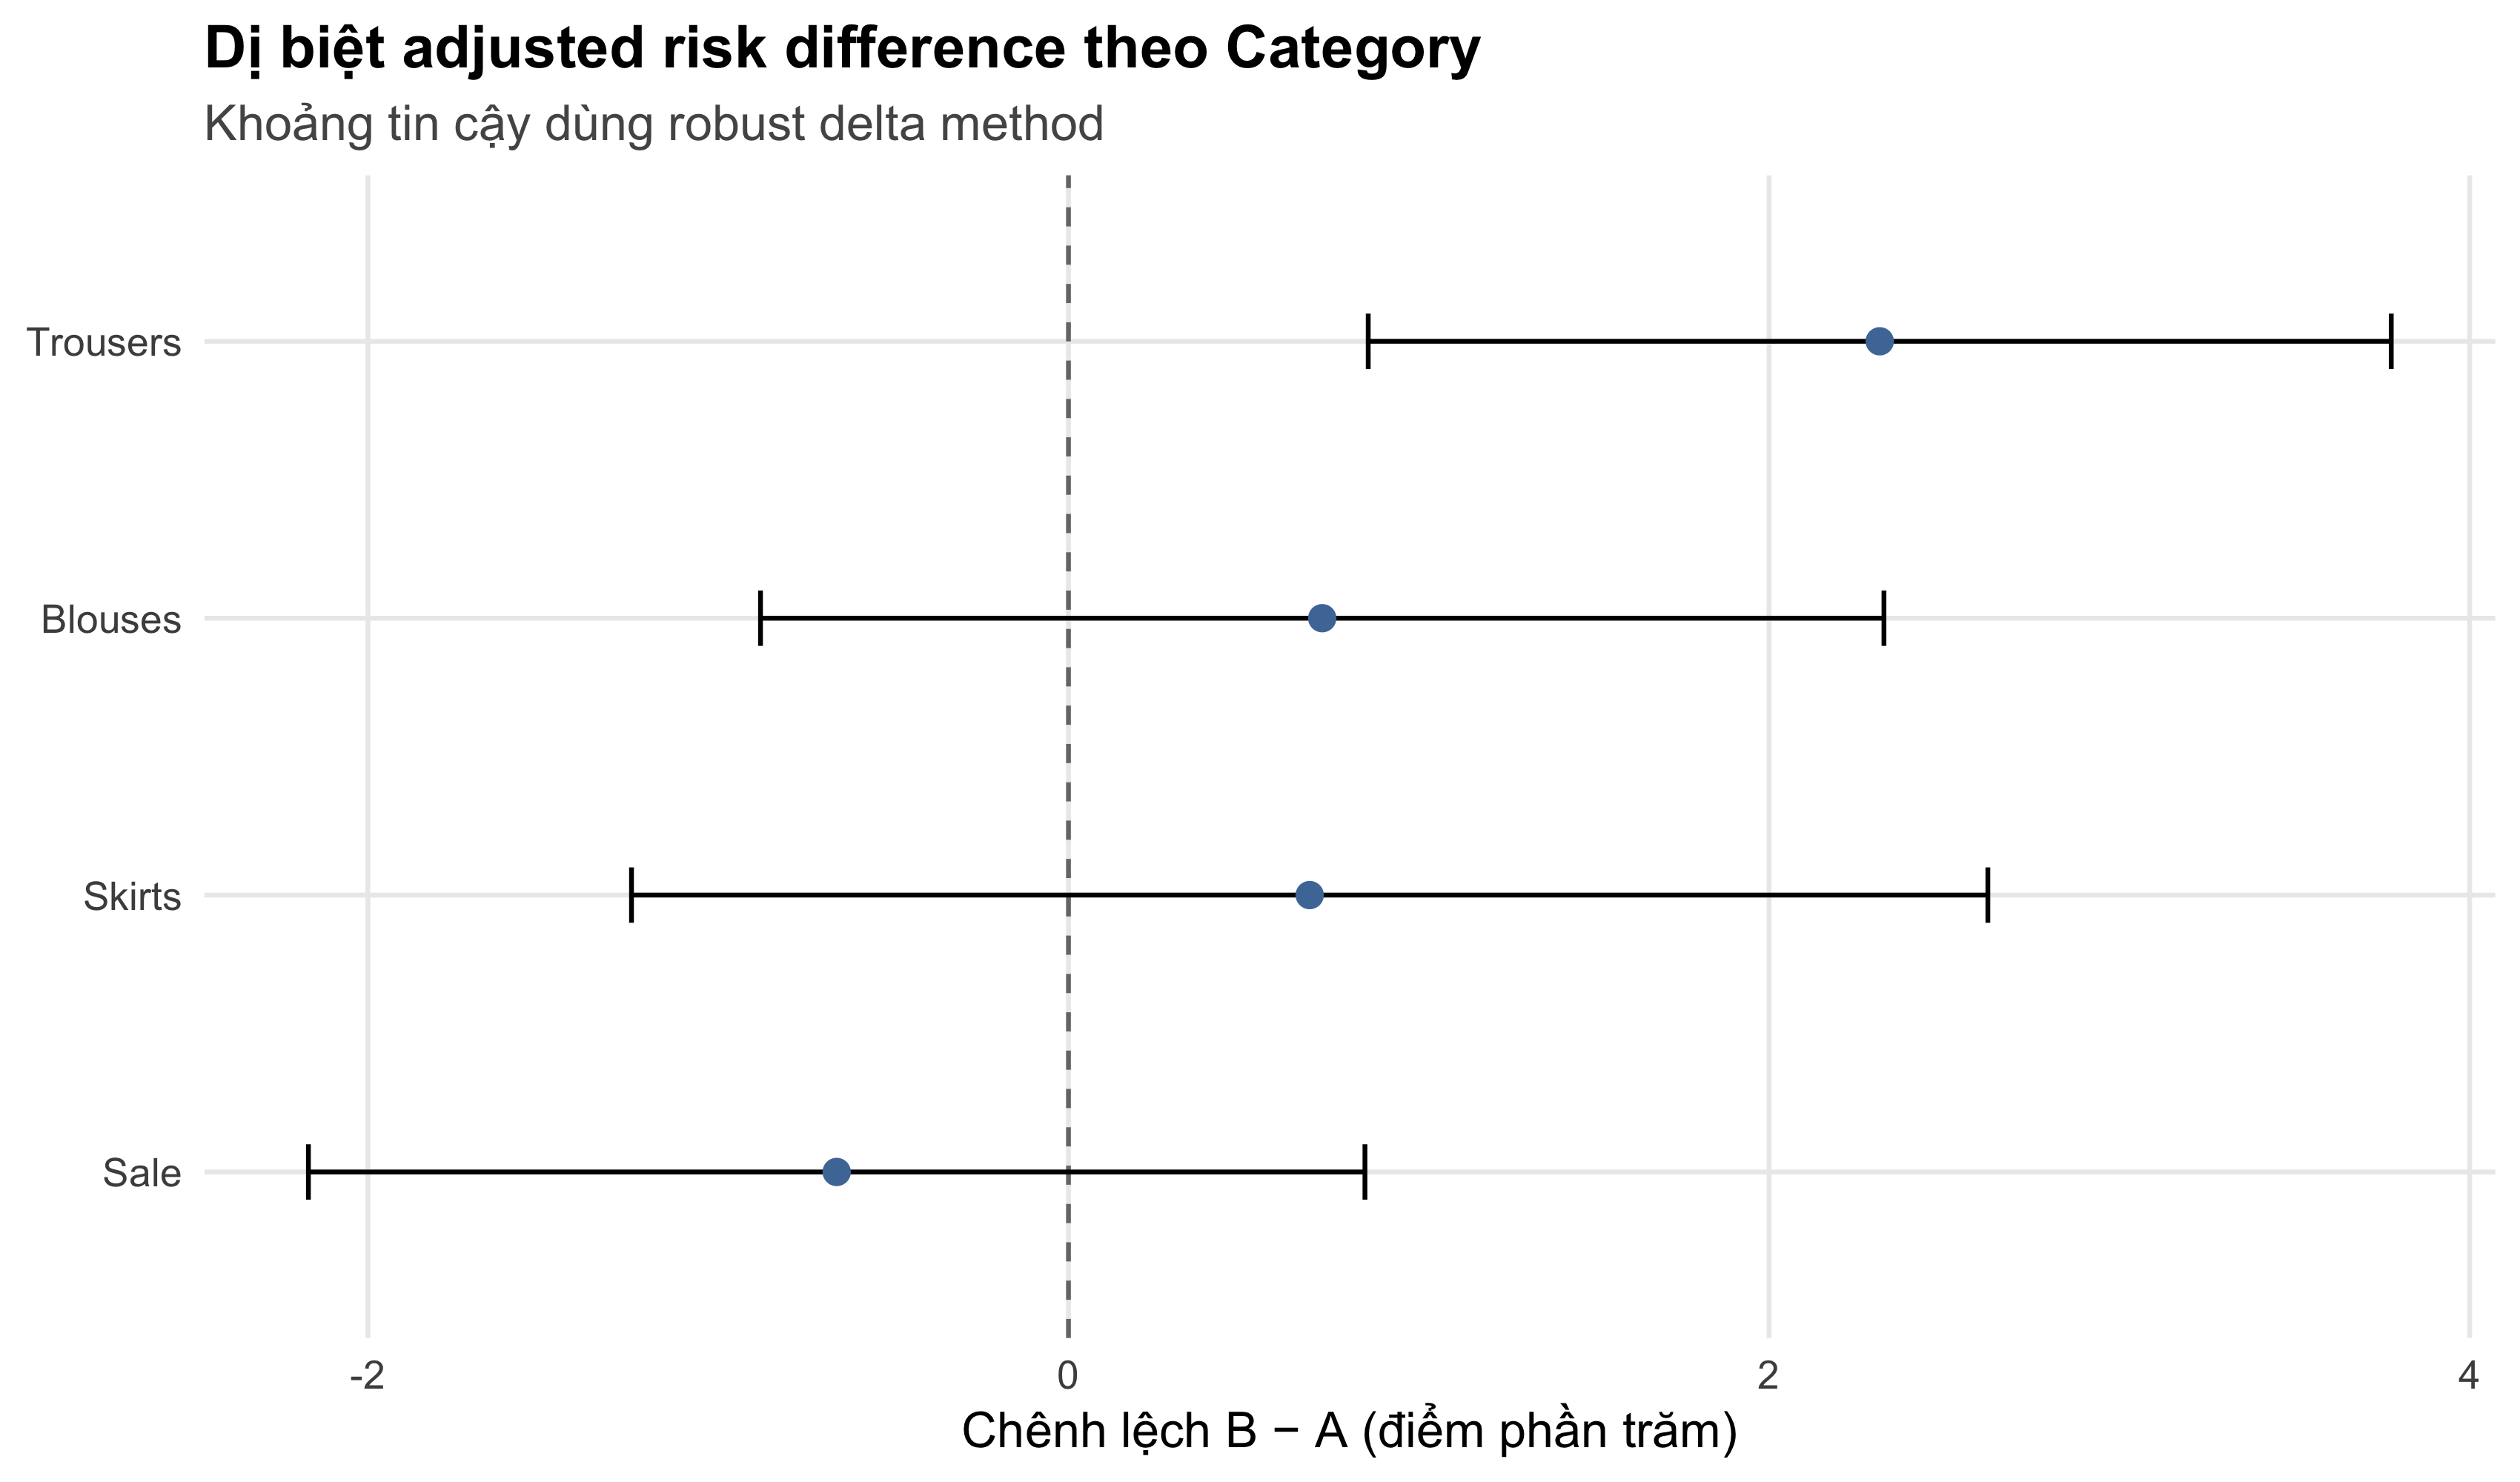
\includegraphics[width=0.85\textwidth]{img/fig-ab-forest.png}
\caption{Forest plot adjusted risk difference của nhóm giá theo danh mục}
\label{fig:ab-forest}
\end{figure}

Kiểm định Wald robust cho toàn bộ nhóm tương tác \texttt{price group} $\times$
\texttt{Category} cho $p = 0{,}051$, tức nằm ngay ranh giới 5\%. Sau hiệu chỉnh
Holm, chỉ riêng danh mục Trousers còn khác biệt có ý nghĩa (2,32 điểm phần trăm,
$p = 0{,}008$); ba danh mục còn lại đều có khoảng tin cậy chứa 0, và Sale thậm
chí có dấu ngược lại. Điều này cho thấy hiệu ứng gộp ở Bảng~\ref{tab:ab-test}
không đại diện đồng đều cho mọi danh mục.

\subsubsection{Độ ổn định theo thời gian}

\begin{table}[H]
\centering
\caption{Độ ổn định theo thời gian của khác biệt giữa hai nhóm giá}
\label{tab:ab-temporal}
\small
\begin{tabular}{lrrll}
\toprule
\textbf{Giai đoạn} & \textbf{Chênh lệch B $-$ A (điểm \%)}
& \textbf{OR điều chỉnh} & \textbf{CI 95\%} & \textbf{p-value} \\
\midrule
Train: tháng 4--6             & 0,78 & 1,066 & 1,032 -- 1,102 & $< 0{,}001$ \\
Phân tích chính: tháng 7      & 1,19 & 1,108 & 1,044 -- 1,175 & $< 0{,}001$ \\
Kiểm tra thời gian: 01--12/08 & 1,36 & 1,125 & 1,021 -- 1,240 & 0,017 \\
\bottomrule
\end{tabular}
\end{table}

Để so sánh nhất quán giữa ba giai đoạn, odds ratio trong
Bảng~\ref{tab:ab-temporal} chỉ điều chỉnh $\log_2(\texttt{order})$, thời gian và
country; vì vậy nó lớn hơn odds ratio 1,071 của mô hình A/B chính -- mô hình đó
còn điều chỉnh thêm toàn bộ đặc điểm sản phẩm nên cho ước lượng thận trọng hơn.

Khác biệt có cùng dấu và độ lớn tương đương trong cả ba giai đoạn, cho thấy đây
là một mối liên hệ ổn định theo thời gian chứ không phải nhiễu ngẫu nhiên của
riêng tháng 7. Tuy nhiên, \texttt{price\_above\_avg} vẫn là một thuộc tính của
sản phẩm chứ không phải treatment được gán ngẫu nhiên, nên kết quả này
\textbf{không} chứng minh rằng tăng giá gây ra việc kết thúc session.

\subsection{Kết quả mô hình dự đoán: xác suất Exit theo tiến trình session}

\begin{table}[H]
\centering
\caption{Tỷ lệ Exit gộp theo khoảng Order trên tháng 7}
\label{tab:hazard}
\small
\begin{tabular}{lrrrl}
\toprule
\textbf{Khoảng Order} & \textbf{Click có nguy cơ} & \textbf{Click kết thúc}
& \textbf{Tỷ lệ Exit} & \textbf{CI 95\%} \\
\midrule
1      & 5.071 & 1.038 & 20,47\% & 19,38\% -- 21,60\% \\
2      & 4.033 & 707   & 17,53\% & 16,39\% -- 18,73\% \\
3--4   & 6.101 & 991   & 16,24\% & 15,34\% -- 17,19\% \\
5--7   & 6.043 & 875   & 14,48\% & 13,61\% -- 15,39\% \\
8--12  & 5.621 & 731   & 13,00\% & 12,15\% -- 13,91\% \\
13--20 & 4.197 & 411   & 9,79\%  & 8,93\% -- 10,73\% \\
$>$20  & 4.165 & 318   & 7,64\%  & 6,87\% -- 8,48\% \\
\bottomrule
\end{tabular}
\end{table}

Xác suất kết thúc giảm gần như đơn điệu theo tiến trình session: từ 20,47\% tại
click đầu tiên xuống 7,64\% với các click sau vị trí 20 -- tức giảm hơn một nửa.
Lưu ý mẫu số ở mỗi hàng là số click \emph{có nguy cơ} trong khoảng đó, không phải
số session ở đầu khoảng; cách tính này tránh diễn giải sai rằng mọi session sống
sót qua click 20 đều có cùng xác suất kết thúc ngay lập tức.

\begin{figure}[H]
\centering
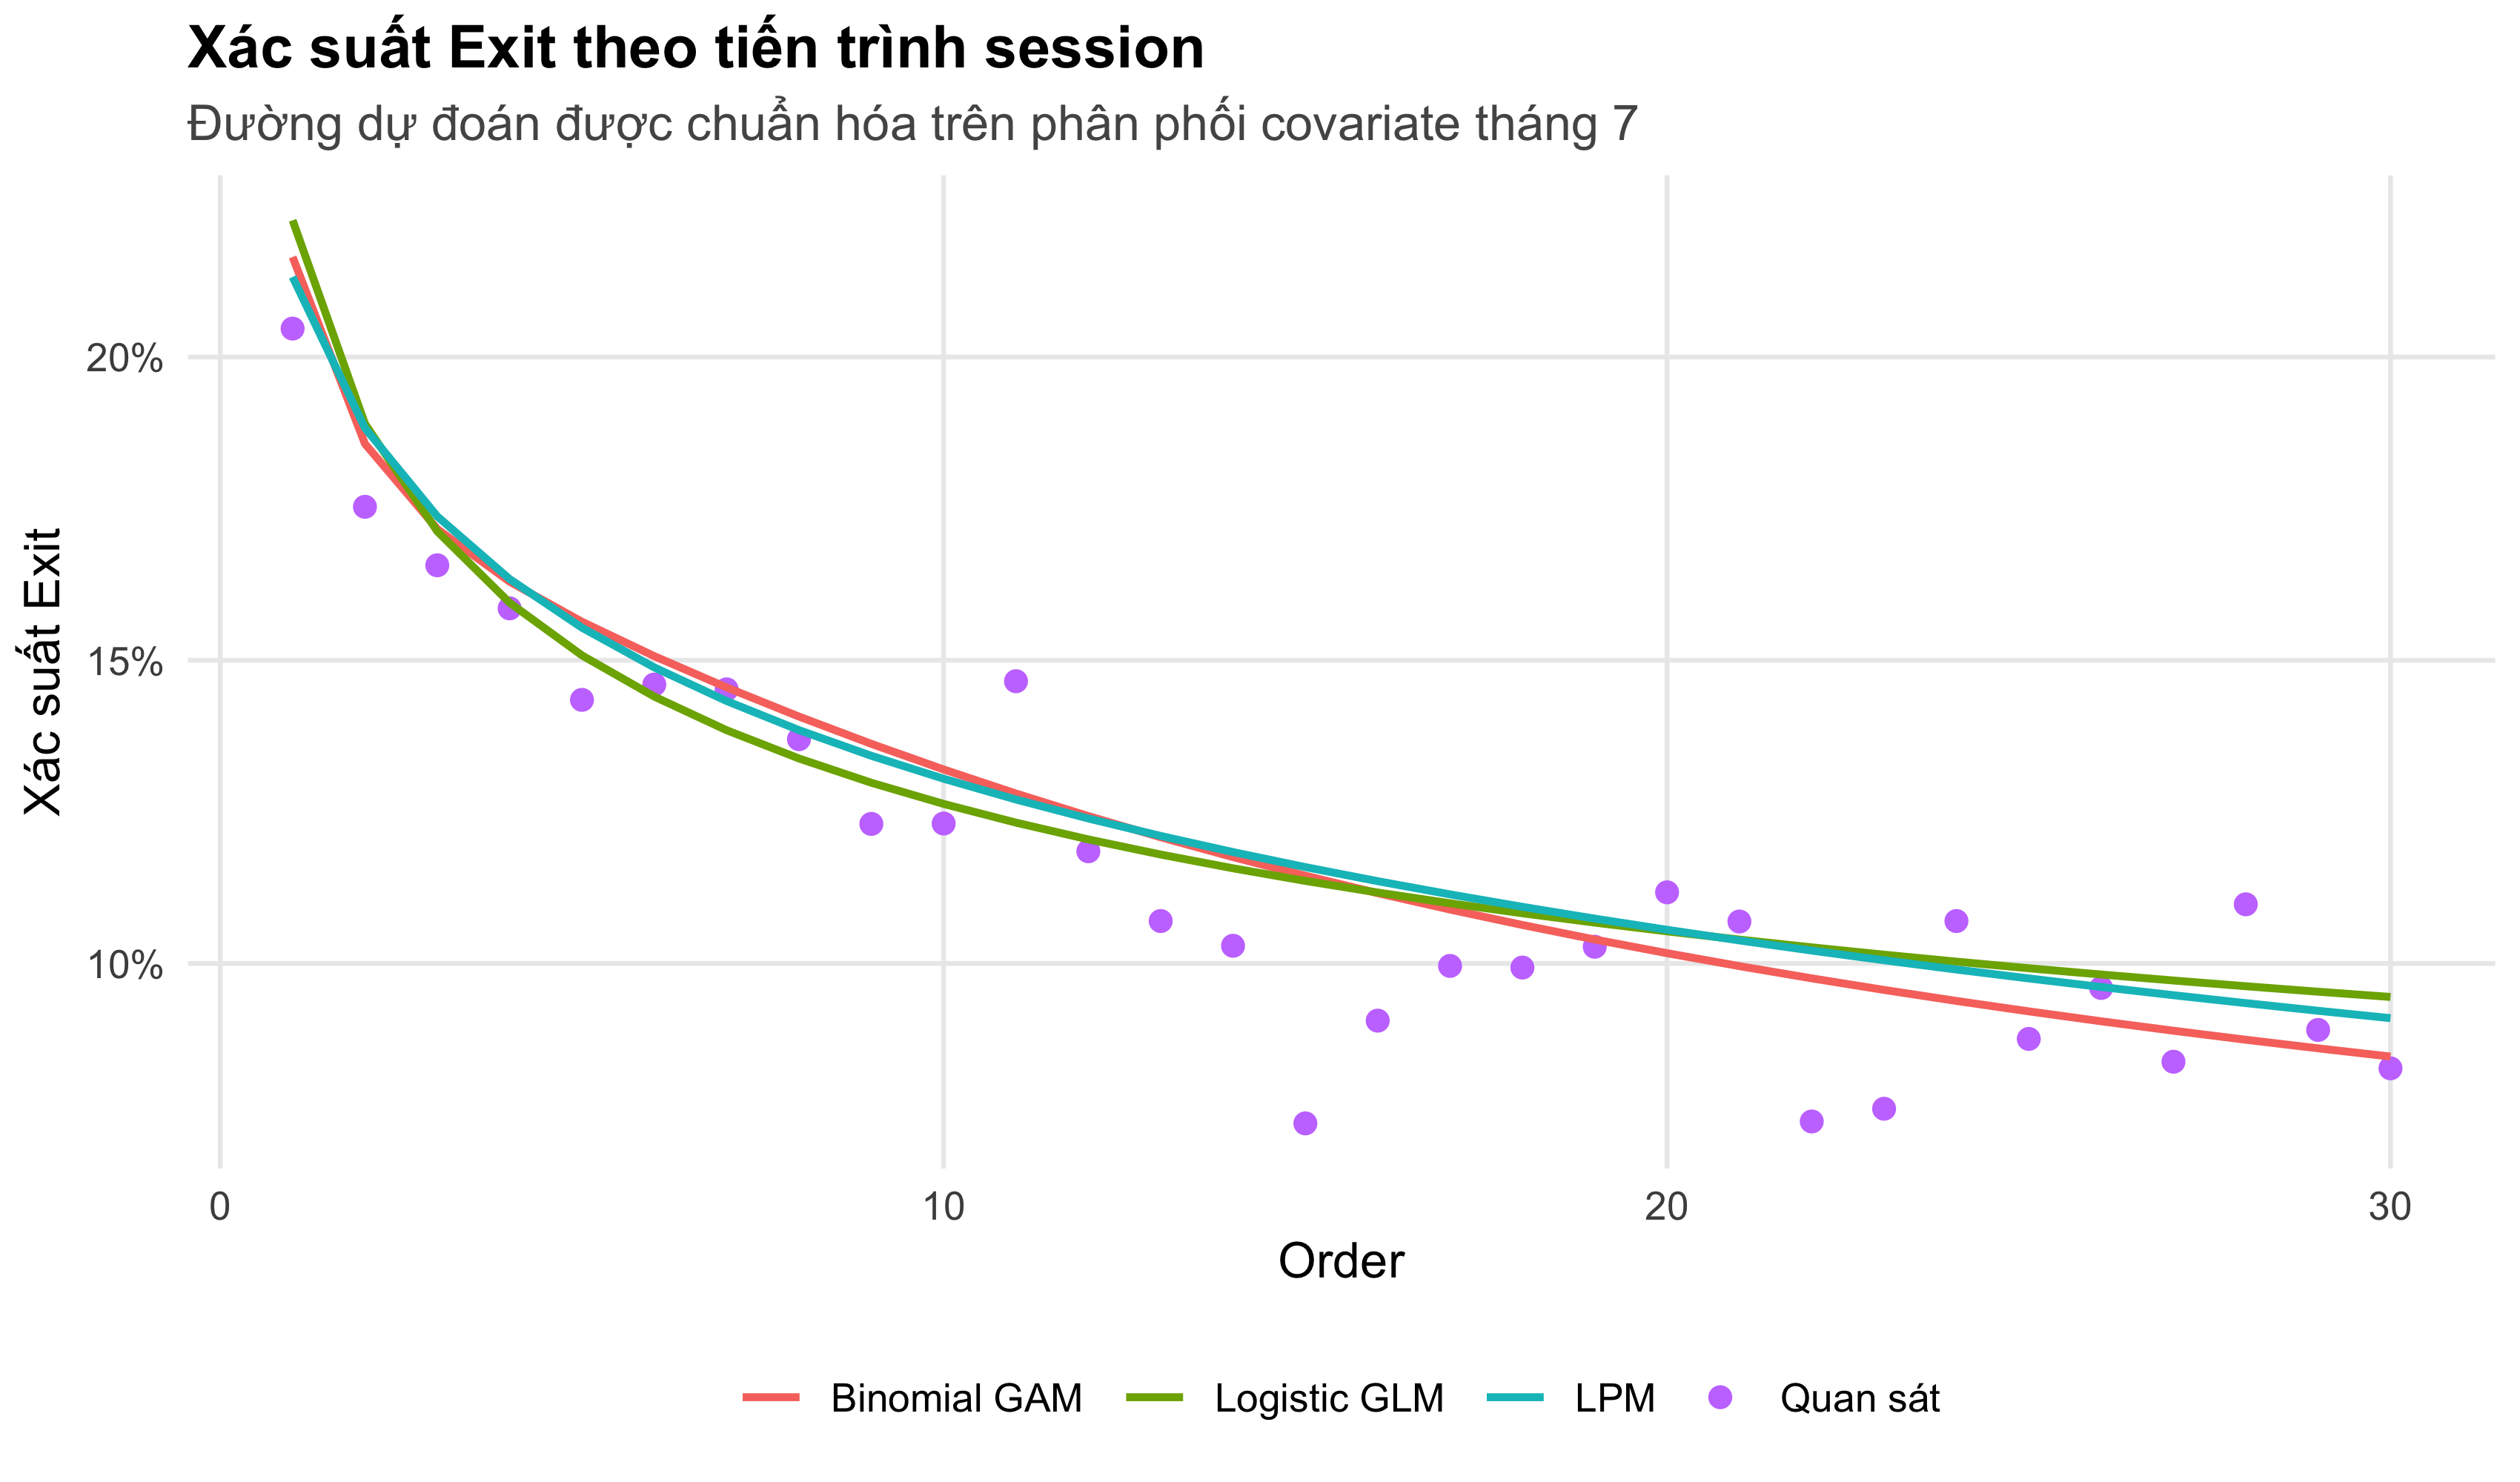
\includegraphics[width=\textwidth]{img/fig-order-probability.png}
\caption{Xác suất Exit quan sát và dự đoán theo tiến trình session; ba đường dự
đoán được chuẩn hóa trên phân phối covariate tháng 7}
\label{fig:order-probability}
\end{figure}

Hình~\ref{fig:order-probability} là căn cứ để trả lời câu hỏi liệu quan hệ tuyến
tính có đủ hay cần đến GAM. Ba đường dự đoán gần như trùng nhau trong khoảng
\texttt{order} từ 1 đến 20; chỉ ở phần đuôi đường GAM mới tách xuống thấp hơn hai
dạng tuyến tính. Nói cách khác, sau phép biến đổi $\log_2$, dạng hàm tuyến tính
đã nắm bắt gần trọn quan hệ và phần phi tuyến còn lại là nhỏ. Các điểm quan sát ở
đuôi dao động mạnh hơn đơn giản vì số session còn tồn tại giảm dần.

\subsection{Kết quả mô hình dự đoán: giá trị bổ sung của các nhóm biến}

Bảng~\ref{tab:model-compare} so sánh chín mô hình (ba phương pháp $\times$ ba
tầng predictor) trên cùng tập validation tháng 7.

\begin{table}[H]
\centering
\caption{So sánh ba tầng predictor của ba phương pháp trên validation tháng 7}
\label{tab:model-compare}
\footnotesize
\setlength{\tabcolsep}{4pt}
\begin{tabular}{llrrrrrrrl}
\toprule
\textbf{Phương pháp} & \textbf{Tầng predictor} & \textbf{ROC--AUC}
& \textbf{AP} & \textbf{Log loss} & \textbf{Brier} & \textbf{Brier skill}
& \textbf{Cal. int.} & \textbf{Cal. slope} & \textbf{AIC} \\
\midrule
LPM      & Baseline         & 0,589 & 0,179 & 0,406 & 0,122 & 0,010 & $-$0,066 & 0,899 & Không so sánh \\
LPM      & Current-click    & 0,611 & 0,197 & 0,405 & 0,121 & 0,016 & $-$0,067 & 0,808 & Không so sánh \\
LPM      & History-enhanced & 0,660 & 0,233 & 0,397 & 0,119 & 0,038 & $-$0,060 & 0,755 & Không so sánh \\
\midrule
Logistic & Baseline         & 0,589 & 0,179 & 0,407 & 0,122 & 0,010 & $-$0,065 & 0,880 & 94.998,4 \\
Logistic & Current-click    & 0,611 & 0,199 & 0,403 & 0,121 & 0,016 & $-$0,068 & 0,873 & 94.222,0 \\
Logistic & History-enhanced & 0,662 & 0,237 & 0,392 & 0,118 & 0,039 & $-$0,059 & 0,922 & 91.801,3 \\
\midrule
GAM      & Baseline         & 0,589 & 0,179 & 0,406 & 0,122 & 0,010 & $-$0,064 & 0,879 & 94.957,6 \\
GAM      & Current-click    & 0,612 & 0,199 & 0,403 & 0,121 & 0,016 & $-$0,067 & 0,864 & 94.160,7 \\
GAM      & History-enhanced & 0,662 & 0,238 & 0,392 & 0,118 & 0,040 & $-$0,057 & 0,932 & 91.746,6 \\
\bottomrule
\end{tabular}

\vspace{4pt}
{\footnotesize AP = Average Precision; Cal. int. = calibration intercept;
Cal. slope = calibration slope. AIC của LPM để trống vì mô hình Gaussian không
cùng họ likelihood với hai mô hình nhị phân nên không so sánh được.}
\end{table}

Cả hai bước bổ sung biến đều có ý nghĩa thống kê. Kiểm định Wald robust chung cho
nhóm \texttt{Price + Category + Colour + Location + Photography + Page} cho
$p < 0{,}001$ trong cả LPM và Logistic GLM. Sau khi đã có các biến current-click,
nhóm biến lịch sử tiếp tục bổ sung với robust joint $p < 0{,}001$.

Điều đáng chú ý là \emph{độ lớn} của hai bước rất khác nhau. Thêm toàn bộ đặc
điểm sản phẩm chỉ nâng ROC--AUC của Logistic GLM từ 0,589 lên 0,611 và giảm log
loss 0,004. Trong khi đó nhóm biến lịch sử duyệt nâng ROC--AUC tiếp lên 0,662 và
giảm log loss thêm 0,012 -- gấp ba lần đóng góp của đặc điểm sản phẩm.\footnote{%
Các mức tăng/giảm được tính trên giá trị chưa làm tròn ($+0{,}050$ ROC--AUC và
$-0{,}012$ log loss), nên có thể lệch một đơn vị ở chữ số thập phân thứ ba so với
hiệu của hai giá trị đã làm tròn trong Bảng~\ref{tab:model-compare}.}
Kết luận thực nghiệm: \textbf{hành vi đã diễn ra trong session mang nhiều thông
tin dự báo hơn hẳn đặc điểm của riêng click hiện tại}.

\begin{table}[H]
\centering
\caption{Mười hai nhóm biến có bằng chứng liên hệ mạnh nhất trong Logistic GLM
history-enhanced (Wald robust theo cụm session)}
\label{tab:terms}
\small
\begin{tabular}{lrrll}
\toprule
\textbf{Nhóm biến} & \textbf{Wald $\chi^2$} & \textbf{df} & \textbf{p-value}
& \textbf{Hiệu ứng / CI 95\%} \\
\midrule
$\log_2(\text{Order})$              & 1081,19 & 1  & $< 0{,}001$ & OR 0,640 (0,623--0,657) \\
Số danh mục duy nhất đến hiện tại   & 639,64  & 1  & $< 0{,}001$ & OR 1,562 (1,509--1,617) \\
Quay lại sản phẩm cũ                & 469,92  & 1  & $< 0{,}001$ & OR 2,218 (2,064--2,384) \\
Page                                & 465,93  & 4  & $< 0{,}001$ & Joint test \\
Country                             & 150,60  & 17 & $< 0{,}001$ & Joint test \\
Colour                              & 93,18   & 13 & $< 0{,}001$ & Joint test \\
Chuyển Category ở click hiện tại    & 75,32   & 1  & $< 0{,}001$ & OR 1,311 (1,233--1,394) \\
Category                            & 48,63   & 3  & $< 0{,}001$ & Joint test \\
Chuyển Page ở click hiện tại        & 46,80   & 1  & $< 0{,}001$ & OR 1,169 (1,118--1,223) \\
Số sản phẩm duy nhất đến hiện tại   & 40,78   & 1  & $< 0{,}001$ & OR 0,988 (0,984--0,991) \\
Location                            & 32,76   & 5  & $< 0{,}001$ & Joint test \\
Price (mỗi 10 USD)                  & 6,96    & 1  & 0,008       & OR 1,032 (1,008--1,056) \\
\bottomrule
\end{tabular}
\end{table}

Năm nhóm biến đứng đầu theo p-value robust và thống kê Wald trên mỗi bậc tự do
là: $\log_2(\text{Order})$, số danh mục duy nhất đã xem, hành vi quay lại sản
phẩm cũ, \texttt{Page} và \texttt{Country}. Ba hiệu ứng đơn biến đáng chú ý:

\begin{itemize}
  \item Mỗi lần \texttt{order} tăng gấp đôi, odds kết thúc session nhân với
  0,640 -- session càng đi sâu càng ít có khả năng dừng ở click kế tiếp.
  \item Click vào một sản phẩm \emph{đã xem trước đó} trong cùng session có odds
  kết thúc cao gấp 2,218 lần, hiệu ứng đơn biến lớn nhất trong mô hình.
  \item Mỗi danh mục mới được xem thêm làm odds kết thúc nhân với 1,562.
\end{itemize}

Ngược lại, \texttt{Price} tuy có ý nghĩa thống kê ($p = 0{,}008$) nhưng hiệu ứng
rất nhỏ: OR 1,032 cho mỗi 10 USD. Cần nhấn mạnh rằng thứ hạng trong
Bảng~\ref{tab:terms} phản ánh \emph{bằng chứng về liên hệ}, không phải mức độ
quan trọng nhân quả, và không nên so sánh trực tiếp độ lớn OR giữa các biến có
đơn vị khác nhau.

\begin{figure}[H]
\centering
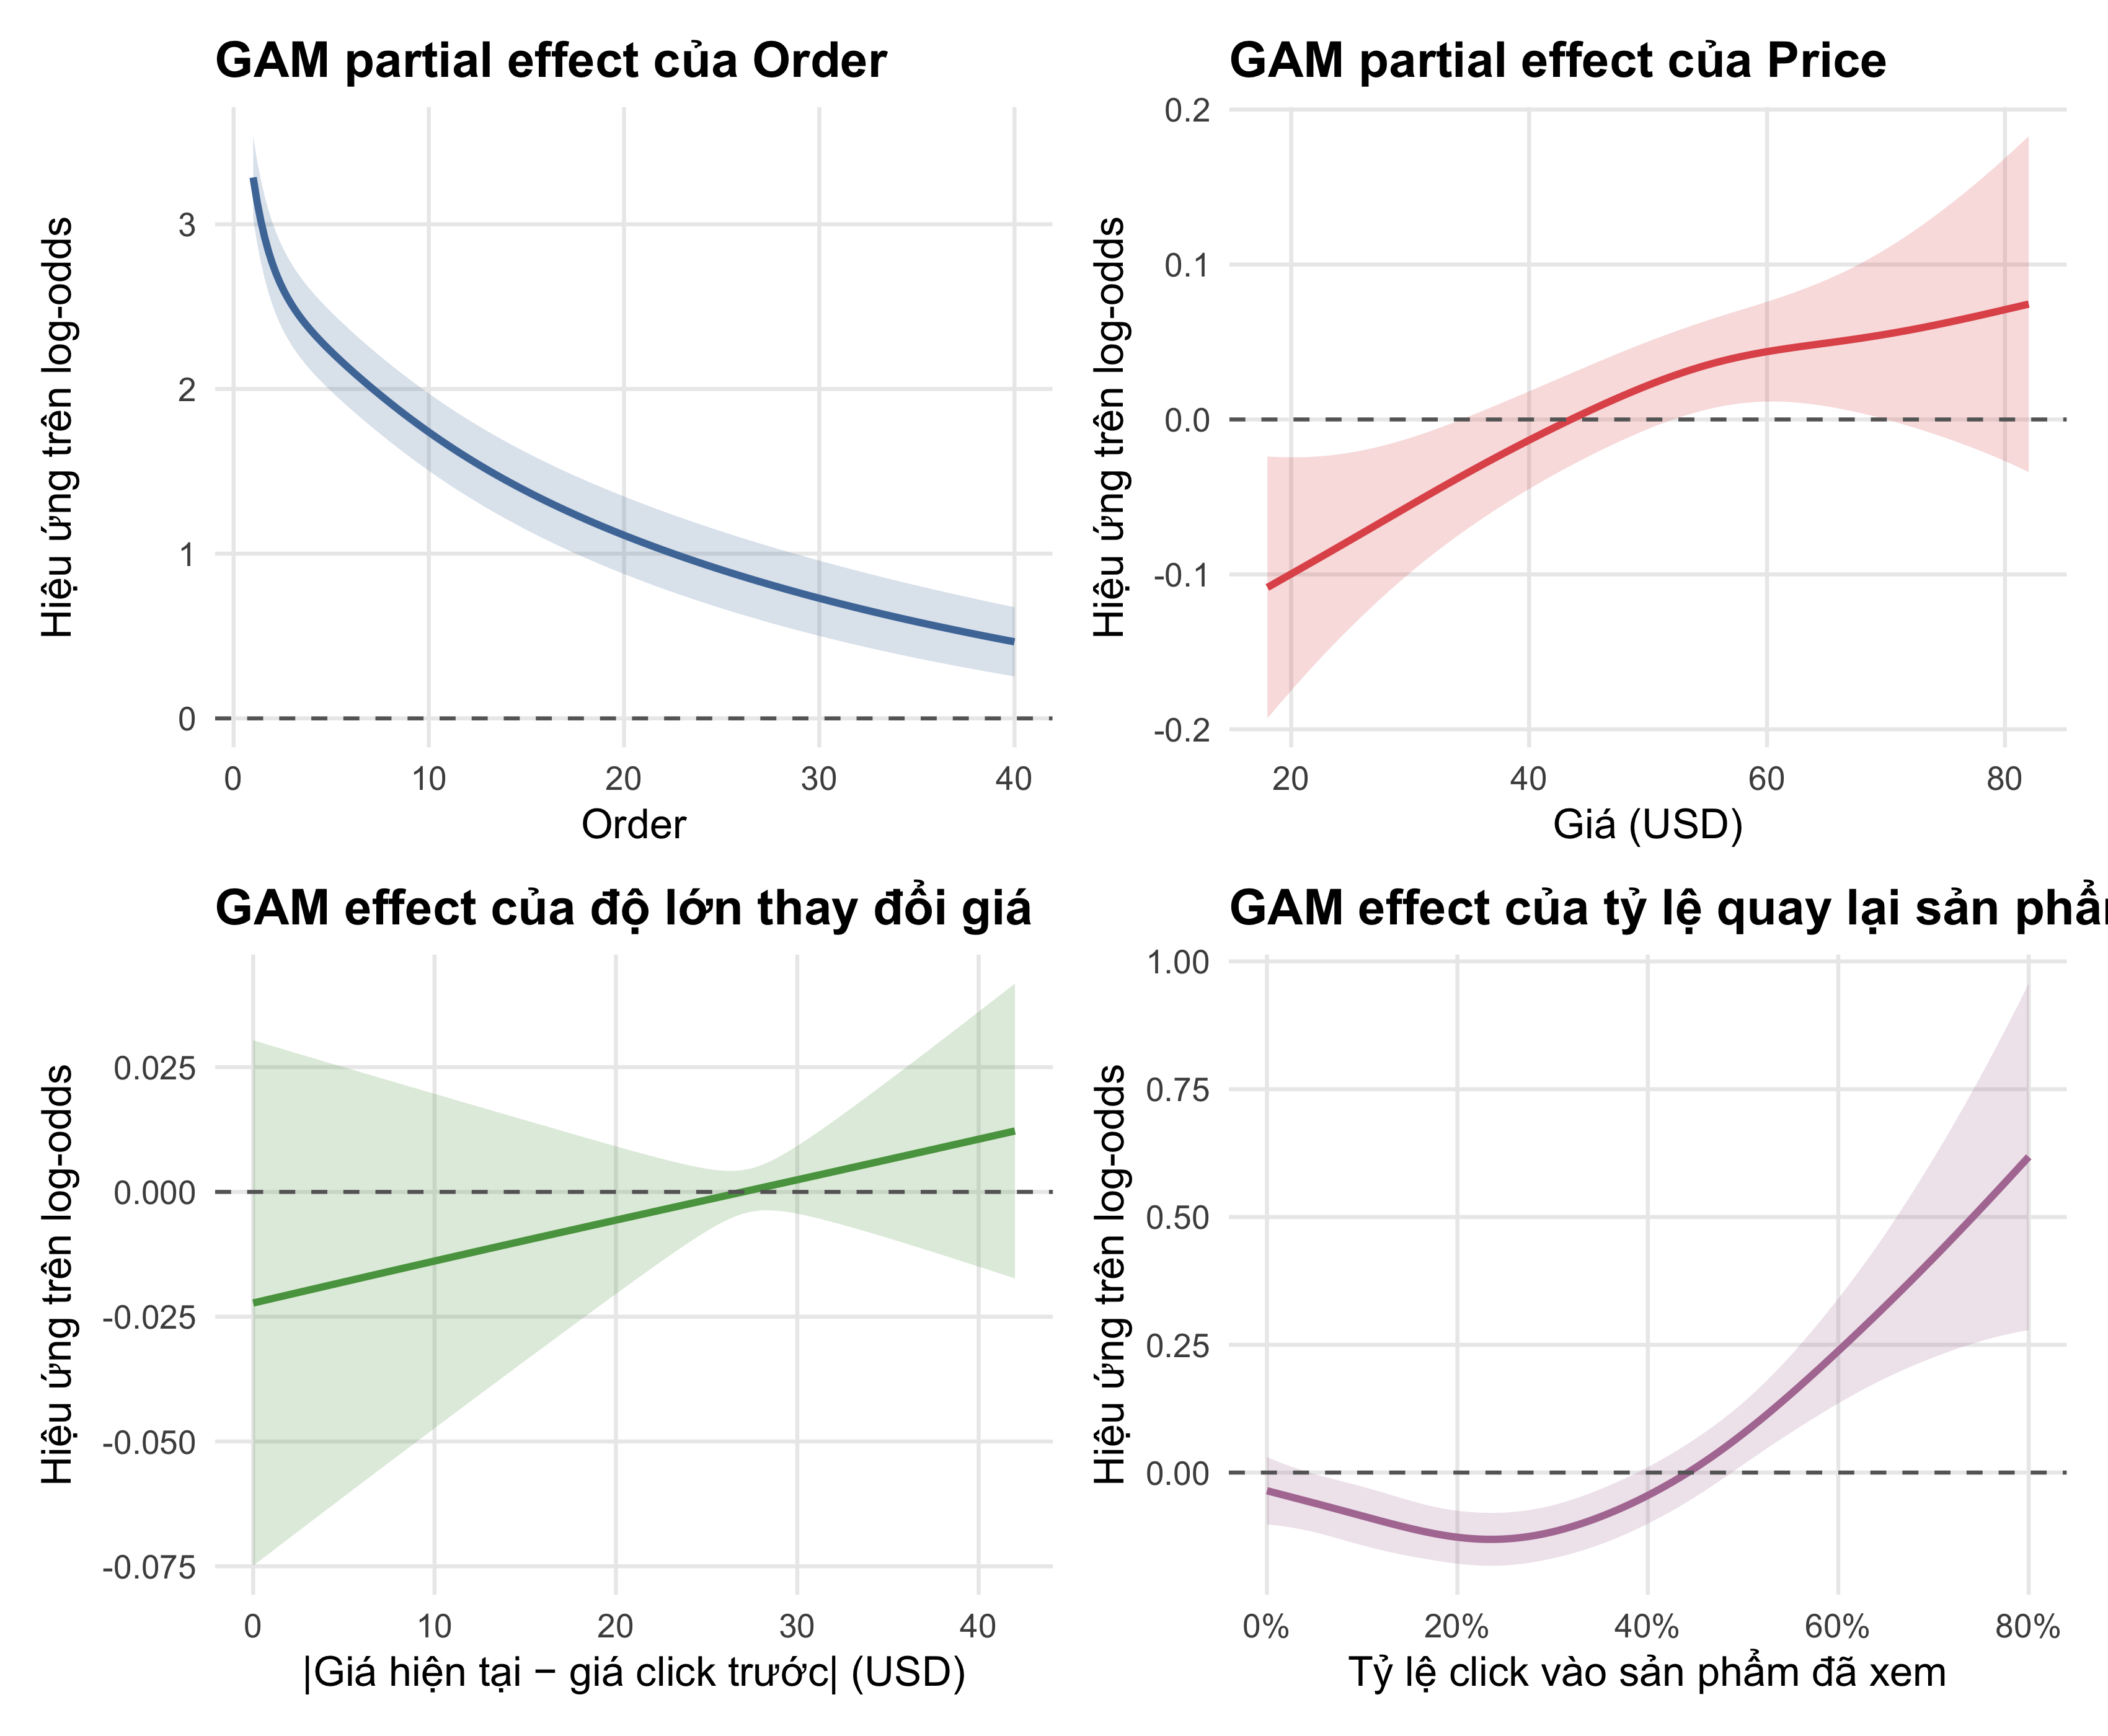
\includegraphics[width=\textwidth]{img/fig-gam-smooths.png}
\caption{Các hàm trơn của GAM history-enhanced: partial effect của Order, Price,
độ lớn thay đổi giá và tỷ lệ quay lại sản phẩm (thang log-odds)}
\label{fig:gam-smooths}
\end{figure}

Hình~\ref{fig:gam-smooths} minh họa dạng hàm mà GAM ước lượng. Hàm trơn của
\texttt{Order} giảm đơn điệu và gần tuyến tính trên thang $\log_2$, phù hợp với
Hình~\ref{fig:order-probability}. Tuy nhiên, như phần chẩn đoán dưới đây chỉ ra,
các partial-effect plot này \textbf{không} được diễn giải như hiệu ứng riêng biệt
của từng biến vì mức concurvity giữa các term rất cao.

\subsection{Chẩn đoán mô hình}

\begin{table}[H]
\centering
\caption{Kiểm tra kích thước basis của GAM history-enhanced}
\label{tab:kcheck}
\small
\begin{tabular}{lrrrr}
\toprule
\textbf{Hàm trơn} & \textbf{$k'$} & \textbf{edf} & \textbf{k-index} & \textbf{p-value} \\
\midrule
s(log2\_order)         & 9,0 & 4,52 & 0,934 & 0,170 \\
s(price)               & 7,0 & 1,88 & 0,943 & 0,350 \\
s(repeat\_rate)        & 7,0 & 3,20 & 0,950 & 0,580 \\
s(abs\_price\_delta\_10) & 7,0 & 1,01 & 0,947 & 0,362 \\
\bottomrule
\end{tabular}
\end{table}

Không hàm trơn nào có edf tiến sát giới hạn basis $k'$ và mọi p-value đều lớn hơn
0,05, nên kích thước basis đã đủ. Đáng chú ý là
$\text{edf} = 1{,}01$ cho \texttt{s(abs\_price\_delta\_10)} và $1{,}88$ cho
\texttt{s(price)} -- hai hàm này gần như tuyến tính, tức GAM hầu như không tìm
thấy phi tuyến đáng kể ở các biến giá.

\begin{table}[H]
\centering
\caption{Mười GVIF điều chỉnh lớn nhất của Logistic GLM (trái) và năm cặp term
có concurvity cao nhất trong GAM (phải)}
\label{tab:collinearity}
\small
\begin{minipage}[t]{0.46\textwidth}
\centering
\begin{tabular}{lr}
\toprule
\textbf{Term} & \textbf{GVIF điều chỉnh} \\
\midrule
log2\_order             & 2,424 \\
unique\_products        & 2,022 \\
price\_vs\_prior\_mean\_10 & 1,989 \\
unique\_categories      & 1,944 \\
price\_10               & 1,729 \\
price\_delta\_10        & 1,688 \\
category\_switch\_rate  & 1,627 \\
repeat\_rate            & 1,497 \\
category\_switch        & 1,442 \\
repeat\_current         & 1,441 \\
\bottomrule
\end{tabular}
\end{minipage}
\hfill
\begin{minipage}[t]{0.50\textwidth}
\centering
\begin{tabular}{llr}
\toprule
\textbf{Term} & \textbf{Term còn lại} & \textbf{Concurvity} \\
\midrule
s(log2\_order)          & para           & 0,994 \\
s(abs\_price\_delta\_10) & para           & 0,966 \\
s(repeat\_rate)         & para           & 0,866 \\
s(log2\_order)          & s(repeat\_rate) & 0,802 \\
para                    & s(repeat\_rate) & 0,769 \\
\bottomrule
\end{tabular}
\end{minipage}
\end{table}

Hai chẩn đoán này cho hai kết luận trái ngược nhau và cần được đọc riêng.
Với Logistic GLM, GVIF điều chỉnh lớn nhất chỉ 2,424, thấp hơn nhiều ngưỡng cảnh
báo thông thường, nên đa cộng tuyến không phải vấn đề với các hệ số trong
Bảng~\ref{tab:terms}. Ngược lại, concurvity trong GAM lên tới 0,994 -- gần mức
xác định hoàn toàn. Nhóm đã loại \texttt{s(unique\_products)} khỏi GAM vì gần
trùng thông tin với \texttt{Order} và \texttt{repeat\_rate}, nhưng concurvity còn
lại vẫn quá cao. Vì vậy GAM chỉ được giữ làm \emph{đối chứng dự báo phi tuyến},
còn các partial-effect plot của nó không được dùng làm bằng chứng về hiệu ứng
riêng của từng biến.

\begin{figure}[H]
\centering
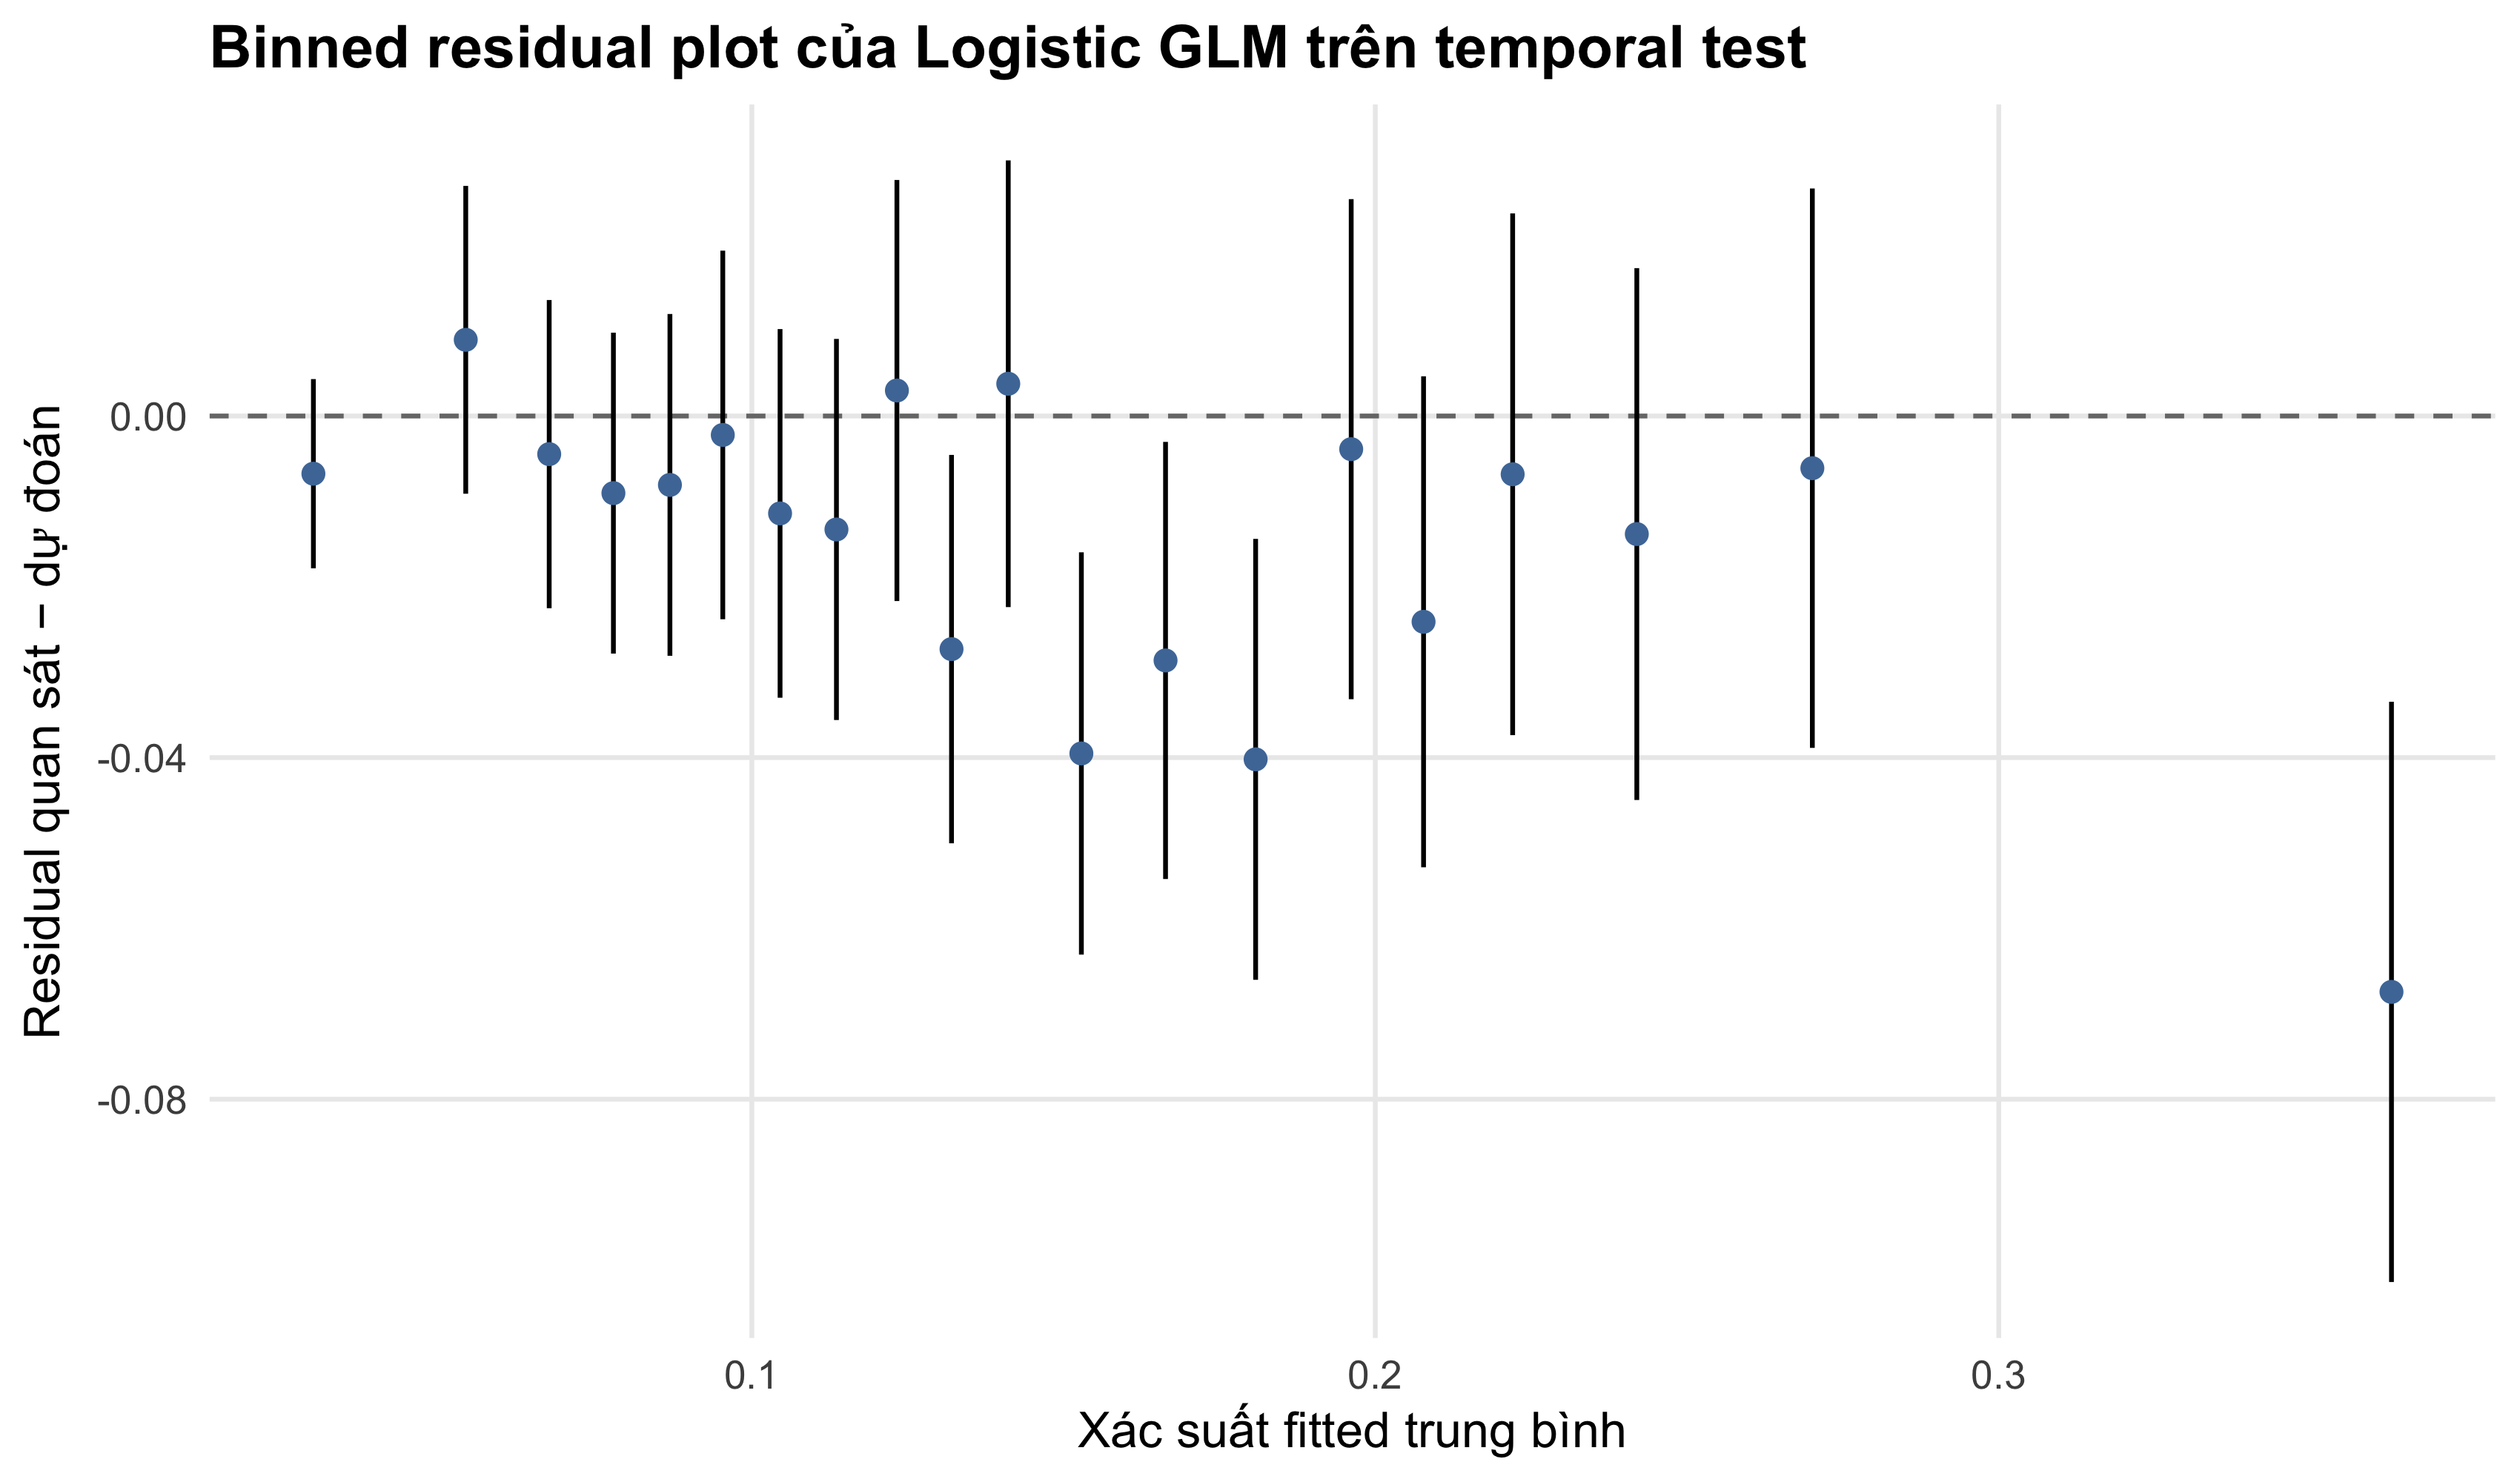
\includegraphics[width=0.85\textwidth]{img/fig-binned-residual.png}
\caption{Binned residual plot của Logistic GLM trên temporal test 01--12/08}
\label{fig:binned-residual}
\end{figure}

Với outcome nhị phân, đồ thị phần dư thông thường của hồi quy tuyến tính không có
ý nghĩa, nên nhóm dùng binned residual plot~\cite{gelman2007}: dữ liệu được chia
thành 20 nhóm theo
xác suất dự đoán và vẽ residual trung bình của mỗi nhóm kèm sai số chuẩn. Phần
lớn các điểm nằm quanh đường 0 với khoảng sai số phủ 0, nghĩa là không có sai
lệch hệ thống rõ rệt theo mức xác suất dự đoán.

\subsection{Kết quả mô hình phân loại: so sánh ba phương pháp}

\subsubsection{Các metric được sử dụng}

Với quan sát $i = 1,\ldots,n$, ký hiệu $y_i \in \{0,1\}$ là nhãn \texttt{Exit}
thực tế và $\hat p_i = P(Y_i = 1 \mid X_i)$ là xác suất do mô hình dự đoán. Báo
cáo đánh giá hai khía cạnh tách biệt: \emph{chất lượng xác suất} và \emph{chất
lượng phân loại sau khi chọn threshold}.

\textbf{Nhóm metric không phụ thuộc threshold.}

\begin{itemize}
  \item \textbf{ROC--AUC} là diện tích dưới đường ROC. Tương đương,
  \[
  \operatorname{AUC} = P(\hat p_{+} > \hat p_{-}) + \tfrac{1}{2}P(\hat p_{+} = \hat p_{-}),
  \]
  với $\hat p_{+}$, $\hat p_{-}$ là xác suất dự đoán của một quan sát dương và
  một quan sát âm lấy ngẫu nhiên. AUC bằng 0,5 tương ứng xếp hạng ngẫu nhiên;
  càng gần 1 càng tốt. Metric này chỉ đo khả năng \emph{xếp hạng}.

  \item \textbf{Average Precision (AP)} tóm tắt đường Precision--Recall,
  $\operatorname{AP} = \sum_k (R_k - R_{k-1}) P_k$. Mốc tham chiếu của mô hình
  ngẫu nhiên xấp xỉ bằng prevalence của \texttt{Exit}. AP được báo cáo cùng AUC
  vì ROC có thể quá lạc quan khi lớp dương chiếm thiểu số.

  \item \textbf{Log loss} đánh giá trực tiếp xác suất dự đoán:
  \[
  -\frac{1}{n}\sum_{i=1}^{n}\left[y_i\log(\hat p_i) + (1-y_i)\log(1-\hat p_i)\right].
  \]
  Càng nhỏ càng tốt; phạt rất nặng các dự đoán tự tin nhưng sai.

  \item \textbf{Brier score} là sai số bình phương trung bình của xác suất,
  $\operatorname{Brier} = \frac{1}{n}\sum_{i=1}^{n}(\hat p_i - y_i)^2$.
  \textbf{Brier Skill Score} so sánh với dự báo hằng bằng prevalence train:
  $\operatorname{BSS} = 1 - \operatorname{Brier}_{model}/\operatorname{Brier}_{ref}$.
  BSS $> 0$ nghĩa là tốt hơn mô hình tham chiếu.

  \item \textbf{Calibration intercept và slope} được ước lượng từ
  $\operatorname{logit}\{P(Y=1)\} = \alpha + \beta\operatorname{logit}(\hat p)$.
  Mô hình hiệu chỉnh lý tưởng có $\alpha = 0$ và $\beta = 1$. Intercept âm cho
  thấy mô hình dự đoán xác suất thiên cao; slope nhỏ hơn 1 cho thấy dự đoán quá
  cực đoan.
\end{itemize}

\textbf{Nhóm metric phụ thuộc threshold.} Sau khi chọn threshold $t$, dự đoán
dương khi $\hat p_i \geq t$. Với $TP, TN, FP, FN$ là số dương đúng, âm đúng,
dương giả và âm giả:

\[
\begin{aligned}
\operatorname{Accuracy} &= \frac{TP+TN}{TP+TN+FP+FN}, &
\operatorname{Precision} &= \frac{TP}{TP+FP}, \\
\operatorname{Recall\ (Sensitivity)} &= \frac{TP}{TP+FN}, &
\operatorname{Specificity} &= \frac{TN}{TN+FP}, \\
F_1 &= 2\,\frac{\operatorname{Precision}\times\operatorname{Recall}}
{\operatorname{Precision}+\operatorname{Recall}}. & &
\end{aligned}
\]

\subsubsection{Lựa chọn mô hình trên validation}

\begin{table}[H]
\centering
\caption{Metric validation tháng 7 dùng để lựa chọn mô hình}
\label{tab:validation}
\small
\begin{tabular}{lrrrrrrr}
\toprule
\textbf{Model} & \textbf{ROC--AUC} & \textbf{AP} & \textbf{Log loss}
& \textbf{Brier} & \textbf{Brier skill} & \textbf{Cal. int.} & \textbf{Cal. slope} \\
\midrule
LPM          & 0,660 & 0,233 & 0,397 & 0,119 & 0,038 & $-$0,060 & 0,755 \\
Logistic GLM & 0,662 & 0,237 & 0,392 & 0,118 & 0,039 & $-$0,059 & 0,922 \\
Binomial GAM & 0,662 & 0,238 & 0,392 & 0,118 & 0,040 & $-$0,057 & 0,932 \\
\bottomrule
\end{tabular}
\end{table}

Quy tắc lựa chọn được xác định \emph{trước} khi nhìn kết quả: giữ lại các mô hình
nằm trong 1\% log loss tốt nhất, rồi trong 1\% Brier tốt nhất; nếu vẫn còn nhiều
ứng viên thì ưu tiên Logistic GLM vì đơn giản và dễ diễn giải hơn GAM, còn LPM
chỉ đóng vai trò benchmark. Logistic GLM và Binomial GAM có log loss và Brier
giống nhau đến ba chữ số thập phân, nên cả hai cùng vào nhóm gần tương đương và
\textbf{Logistic GLM được chọn}. Threshold tối đa $F_1$ của từng mô hình được
chốt từ prediction out-of-fold của five-fold CV theo session trên tập train,
trước khi mở temporal test.

\subsubsection{Hiệu năng cuối trên temporal test}

\begin{table}[H]
\centering
\caption{Hiệu năng cuối của ba mô hình trên temporal test 01--12/08; khoảng tin
cậy 95\% từ 500 lần cluster bootstrap theo session}
\label{tab:final-metrics}
\footnotesize
\setlength{\tabcolsep}{4pt}
\begin{tabular}{llllrlrrr}
\toprule
\textbf{Model} & \textbf{ROC--AUC} & \textbf{AP} & \textbf{Log loss}
& \textbf{BSS} & \textbf{Brier} & \textbf{Cal. int.} & \textbf{Cal. slope}
& \textbf{Ngoài $[0,1]$} \\
\midrule
LPM          & 0,662 (0,644--0,681) & 0,224 (0,212--0,241) & 0,382 (0,363--0,399) & 0,036 & 0,114 (0,107--0,120) & $-$0,138 & 0,868 & 1,706\% \\
Logistic GLM & 0,666 (0,647--0,685) & 0,230 (0,218--0,246) & 0,379 (0,361--0,396) & 0,039 & 0,113 (0,107--0,119) & $-$0,127 & 0,934 & 0,000\% \\
Binomial GAM & 0,666 (0,647--0,686) & 0,230 (0,218--0,247) & 0,379 (0,361--0,396) & 0,039 & 0,113 (0,107--0,119) & $-$0,125 & 0,942 & 0,000\% \\
\bottomrule
\end{tabular}
\end{table}

Ba mô hình gần như không phân biệt được về khả năng xếp hạng: khoảng tin cậy
ROC--AUC chồng lấn gần hoàn toàn. Khác biệt thực chất nằm ở hai chỗ khác. Thứ
nhất, \textbf{calibration slope}: LPM chỉ đạt 0,868 trong khi Logistic GLM đạt
0,934 và GAM đạt 0,942 -- xác suất của LPM cực đoan hơn mức dữ liệu cho phép.
Thứ hai, \textbf{tính hợp lệ của xác suất}: LPM sinh ra 1,706\% dự đoán nằm ngoài
khoảng $[0,1]$, tức những giá trị không thể diễn giải như xác suất; hai mô hình
nhị phân theo cấu trúc không bao giờ mắc lỗi này.

Brier Skill Score của cả ba mô hình chỉ nằm trong khoảng 0,036--0,039, nghĩa là
chúng chỉ tốt hơn dự báo hằng bằng prevalence khoảng 4\%. Đây là mức cải thiện
khiêm tốn và cần được nêu rõ thay vì che đi sau con số AUC.

\begin{figure}[H]
\centering
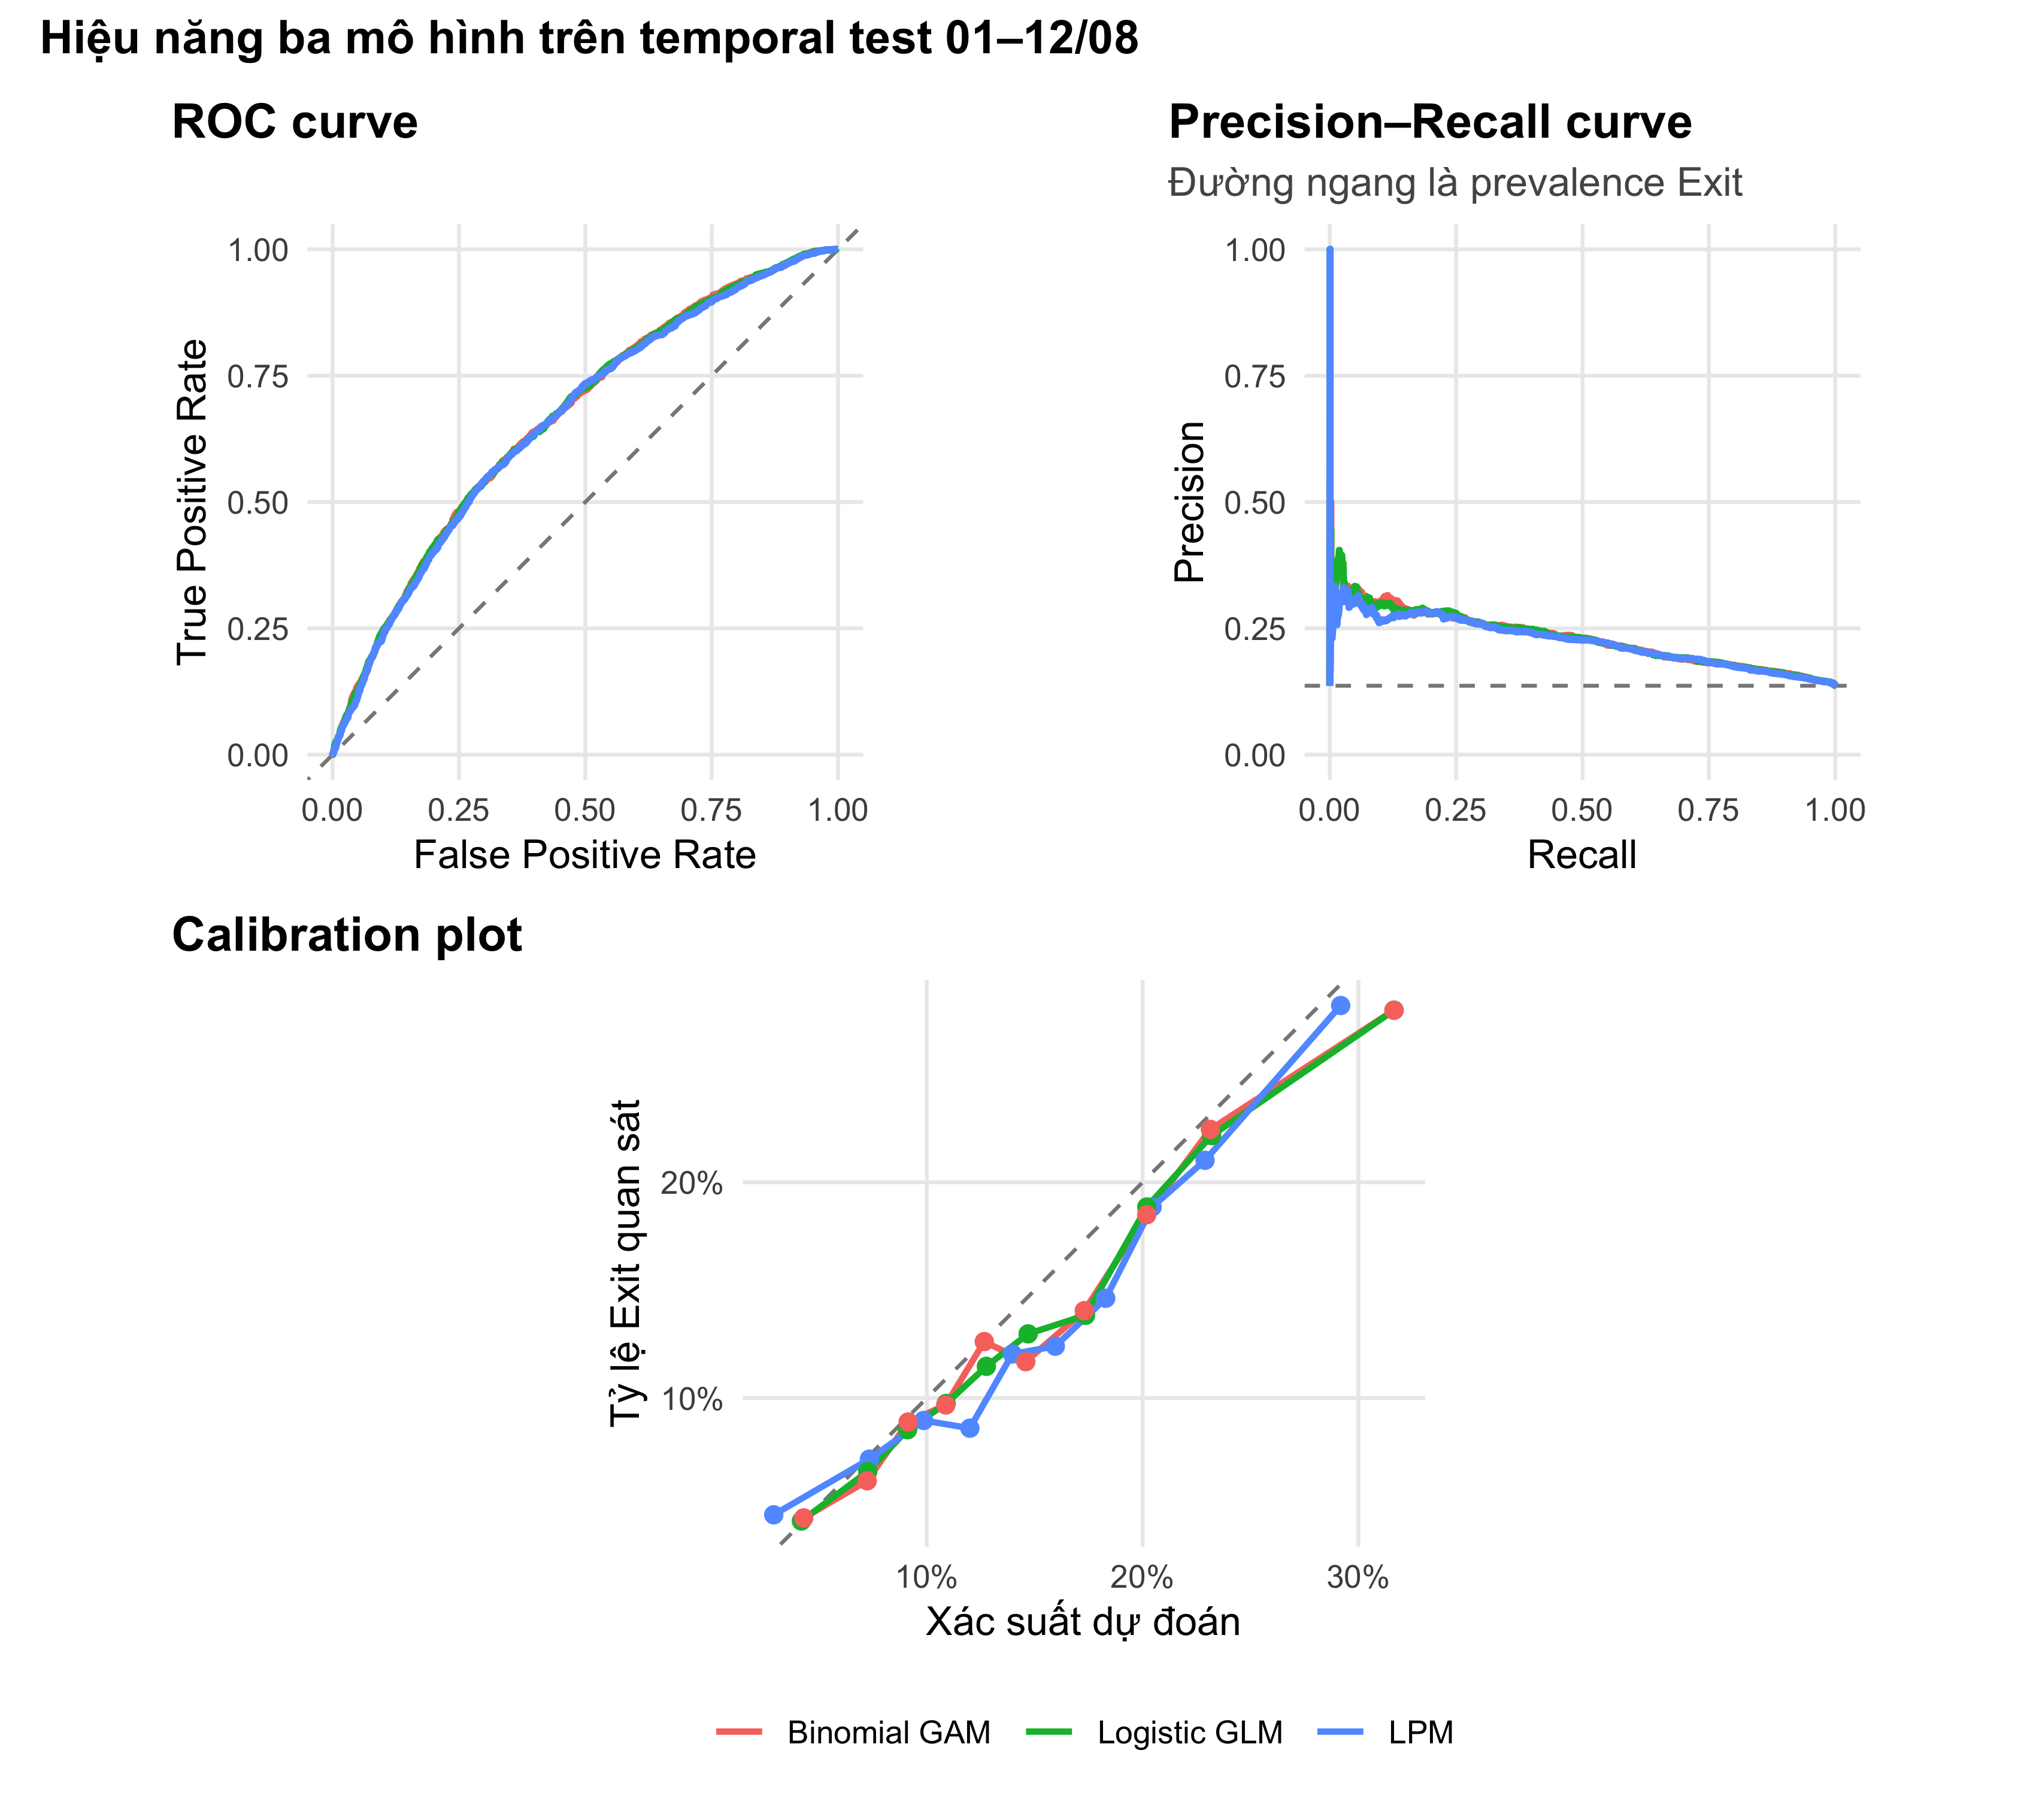
\includegraphics[width=0.95\textwidth]{img/fig-roc-pr-calibration.png}
\caption{Đường ROC, đường Precision--Recall và calibration plot của ba mô hình
trên temporal test 01--12/08. Đường đứt nét là mốc tham chiếu: xếp hạng ngẫu
nhiên (ROC), prevalence Exit (PR) và hiệu chỉnh hoàn hảo (calibration)}
\label{fig:roc-pr-calibration}
\end{figure}

\begin{table}[H]
\centering
\caption{Ma trận nhầm lẫn và các metric phân loại trên temporal test, tại
threshold đã khóa từ prediction out-of-fold của train}
\label{tab:classification}
\small
\setlength{\tabcolsep}{5pt}
\begin{tabular}{lrrrrrrrrrr}
\toprule
\textbf{Model} & \textbf{Threshold} & \textbf{TP} & \textbf{TN} & \textbf{FP}
& \textbf{FN} & \textbf{Accuracy} & \textbf{Precision} & \textbf{Recall}
& \textbf{Specificity} & \textbf{F1} \\
\midrule
LPM          & 0,168 & 1.176 & 7.428 & 4.617 & 727 & 61,69\% & 20,30\% & 61,80\% & 61,67\% & 30,56\% \\
Logistic GLM & 0,162 & 1.145 & 7.722 & 4.323 & 758 & 63,57\% & 20,94\% & 60,17\% & 64,11\% & 31,07\% \\
Binomial GAM & 0,163 & 1.123 & 7.843 & 4.202 & 780 & 64,28\% & 21,09\% & 59,01\% & 65,11\% & 31,07\% \\
\bottomrule
\end{tabular}
\end{table}

Các threshold được chọn (0,162--0,168) đều thấp hơn 0,5 rất nhiều, đúng như kỳ
vọng với dữ liệu mất cân bằng. Tại các ngưỡng này, cả ba mô hình đều có
Recall khoảng 59--62\% nhưng Precision chỉ khoảng 21\%: cứ 5 click bị dự báo là
kết thúc thì chỉ khoảng 1 click thực sự kết thúc. $F_1$ tối đa chỉ đạt 31,07\%.
Accuracy từ 61,69\% đến 64,28\% \emph{thấp hơn} mức 85,48\% mà một mô hình luôn dự đoán
``Continue'' đạt được -- minh chứng cụ thể cho lý do Accuracy không được dùng làm
tiêu chí chọn mô hình ở đây.
